% SPDX-License-Identifier: CC-BY-4.0
%
% Copyright (c) 2023 Nelson Vieira
%
% @author Nelson Vieira <nelson0.vieira@gmail.com>
% @license CC-BY-4.0 <https://creativecommons.org/licenses/by/4.0/legalcode.txt>
\section{Methodology} \label{section:methodology}

The overall work is comprised of two phases which will be described
in the following paragraphs. The first phase, which is primarily described
on Chapter \ref{section:state_of_the_art}, focuses on gathering the state
of the art in terms of the most relevant topics, from which the main privacy
concepts were selected to be explored in the first stage of phase two with
the creation of a questionnaire with the aim to collect user perceptions
of privacy. The second stage of phase 2 consisted in developing an
application, partially based on the information generated by the survey,
that can identify what sort of devices are around, what kind of data is
gathered by these devices, present privacy options to the user when available,
and what can be done to prevent undesirable data from being collected.
\par
The first phase involved conducting a systematic literature review to gather
the most relevant papers discussing methodologies and techniques for the
protection of user privacy data with a focus on IoT systems. This SLR focused
on papers from the last 13 years, from 2010 until 2023, since papers
published prior to 2010 become out of date with the evolution of technology.
Although certain aspects of privacy have remained constant throughout the years,
this historical perspective on privacy is primarily discussed in the
introduction to this work.

The SLR followed Keshav's three-pass approach \cite{KeshavHow} and
PRISMA 2020 \cite{pagen2021prisma} guidelines when selecting the papers
for review, the principles suggested by Kitchenham and Charters \cite{kitchenham2007guidelines}
were also taken into account in order to ensure the transparency and
reliability of the review. On Keshav's approach, first the title would
be read, then the abstract, the introduction and conclusion and briefly
skim the rest of the paper and then decide if it was worth reading any
further. If the document passed the inclusion criteria, which will be
discussed further ahead, then the document would be read in its entirety
while ignoring any tables, figures, images or graphs. If the paper failed
to present any interesting idea, approach, or technique it would be discarded,
but if not, it would be read carefully from the beginning again in order
to fully understand what it presents.
% Figure \ref{} represents this process.

It is challenging to curate the literature and
gain an in-depth understanding of its different aspects due to the vast
array of approaches that address the topic IoT privacy. As a result, specific
databases were used because of the sheer quantity of papers contained within
them makes research easier. The following were the primary databases of the SLR:

\begin{itemize}
    \item[$\bullet$]
    Google Scholar;
    \item[$\bullet$]
    ScienceDirect;
    \item[$\bullet$]
    IEEE Explore Digital Library;
    \item[$\bullet$]
    ResearchGate;
    \item[$\bullet$]
    Elicit;
    \item[$\bullet$]
    BASE.
\end{itemize}

Other supplementary databases used, during the course of the research, include:
CORE, AIS, ACM Digital Library, Semantic Scholar, Baidu Scholar, RefSeek and
Science.gov. These databases were used in to search certain works that
would have not been found otherwise.

The papers were collected by searching the databases with keywords, a broad
spectrum of results were obtained using generic terms like. The primary search
terms were used between quotation marks, e.g. ``Internet of Things'', so that
results include all words in sequence, operators AND and OR were also used
as was a minus sign before a keyword to remove said keyword from the search
results. Many search terms were utilized, however the most often
used ones, based on their frequency, include: ``Digital literacy'',
``Differential privacy'', ``Privacy paradox'', ``Machine learning'',
``Blockchain'', ``User awareness'', ``User knowledge'', ``Blockchain'',
``Privacy concerns'', ``Privacy perceptions'', ``Regulation'',
``Framework'', ``Security'', ``Deep learning'', ``Approach''.
Most of these search terms also included the terms ``Privacy'' and/or
``Internet of Things'' or any variants like ``IoT'' or ``IoT privacy''.

The SLR attempts to summarize and evaluate IoT privacy concerns, as well
as ideas, techniques, or methodologies to overcome those challenges.
The focal point in this phase was answering the following question: Does
the paper present a new methodology or interesting angle to tackle users'
privacy concerns?
% A better restatement of inclusion criteria is formulated
% in the following research questions:\\

% \vspace{5mm}
% \textbf{Phase 1 (Literature review):} \\

% \textbf{RQ1:} What approaches are currently being considered to address privacy
% issues in IoT?

% \textbf{RQ2:} What issues are prevalent in IoT that make it challenging to
% protect individuals privacy? \\

As referenced before, only papers published from 2010 until 2023 are considered,
these works must also be published in journals, conference proceedings, dissertations,
thesis or technical reports. Exclusion criteria include: presentations, editorials,
abstracts or commentaries. Works can cover any area as long as they deal with
privacy in the Internet of Things, if the paper does not cover IoT then at least
it must cover privacy aspects that can be applied to IoT, as is the case of the
privacy paradox.

From database searches, a total of 229 papers were found. Applying the inclusion
and exclusion criteria to these papers bring the total number of papers down to
95, excluding 134 papers. After reading the full texts of the remaining 95 papers,
47 were excluded, making the number of total papers in the SRL be 48.

Having collected the major findings of the SLR, this work then aimed to conduct a
throughout study split into two stages, which will compose phase 2 of this work.
% The following research questions will be made for this phase:\\

% \vspace{5mm}
% \textbf{Phase 2 (Survey and application):} \\

% \textbf{RQ3:} What are the perceptions of individuals on online privacy?

% \textbf{RQ4:} How can users be empowered to protect their privacy in IoT systems?\\
% \vspace{5mm}

The second phase was evaluated on two stages, the first one consisted
on doing a questionnaire on people's general privacy concerns, while using and interacting
with IoT devices. The SLR helped on the creation of the questionnaire to
assess general user's knowledge on privacy concepts, their habits and concerns,
their understanding of privacy rights, and what they do to safeguard those
rights. The goal of this study was to both understand the privacy paradox
and collect insights on how to address privacy issues in IoT devices.

% Having collected the major findings, this work then aims to conduct a throughout
% study split in several stages and around the following research questions:

% \textbf{RQ1:} What approaches are being considered for privacy issues in
% IoT in the currently available literature?

% \textbf{RQ2:} What IoT-related tools are available that empower users to
% protect their privacy rights? OR How to empower users to protect their privacy
% rights?

% \textbf{RQ3:} What issues are prevalent in IoT that make it difficult to
% address privacy and security problems?

% The proposed methodology is composed of two phases, the first phase consists
% on doing a study on people's general privacy concerns while using and interacting
% with IoT devices. This study will consist on preparing a questionnaire to
% assess general user's knowledge on privacy concepts, their habits and concerns,
% their understanding of privacy rights, and what they do to safeguard those
% rights. The goal of this study is to both understand the privacy paradox
% and collect data on their proposal to address privacy issues with regard
% to IoT devices. The second phase consists in developing an application, partially
% based on the information generated by the survey, that can identify what sort
% of devices are around, what kind of data is gathered by these devices, present
% privacy options to the user where available, and what can be done to prevent
% undesirable data from being collected.

% The second phase consists
% in doing an application that can detect IoT devices nearby the user with.
% The application should do the following when
% detecting a device:
% 1. it should show some information about the device;
% 2. it should categorize the device;
% 3. it should provide the user with privacy options, if the device allows the
% user to decline data harvesting.
% This application at first sight might appear to be a mere privacy assistant
% but it's not, because IoT assistants merely choose what privacy options the
% user first sets and maintains it for every other application that the user
% might use. The proposed app doesn't have the objective to conform to the user's
% preferred privacy choices, it merely informs the user about nearby IoT devices
% and can provide the user with privacy options. But the main objective is creating
% awareness in individuals about the various devices that are around and make
% the user questions their choices.

\subsection{Stage 1: User perceptions}

This questionnaire aims to understand people's perception of IoT and their privacy
practices online. It also serves to better understand and demystify the privacy
paradox and to help provide a solution to the privacy issue in IoT, which will be
discussed on Section \ref{subsection:stage2}.

The questionnaire consisted of 86 questions divided into 7 sections to
gauge users' digital literacy, the first section being about general privacy
questions, then about the predisposition to data sharing, to concerns with
privacy then about daily digital routines, then about profile identification,
subsequently about IoT general knowledge before a final part about
non-identifiable demographic data. The questionnaire's structure is shown
in more detail in Table \ref{table:questionnaire}, the full questionnaire
is presented on Appendix \ref{appendix:survey}.

\begin{table}[H]
    \begin{center}
        \begin{tabular}{r *{3}{ p{6cm} }}
            \hline
            $\#$\hspace{0.5cm} & Section & Details \\
            \hline
            1\hspace{0.5cm} & General knowledge and attitudes towards privacy & This
            section's goal is to ask generic questions regarding the participants awareness
            of information privacy. \\
            \hline
            2\hspace{0.5cm} & Disposition for sharing personal information & This
            section is designed to elicit generic inquiries about the participants
            willingness to provide personal information. \\
            \hline
            3\hspace{0.5cm} & Privacy concerns & This section strives to
            elicit questions about potential concerns about disclosing
            personal information. \\
            \hline
            4\hspace{0.5cm} & Current online habits and practices & This
            section includes general questions with regard to working with
            the internet in everyday activities. \\
            \hline
            5\hspace{0.5cm} & Profile identification & This section gathers
            more particular questions concerning employing profiles to make
            it more straightforward to generate tailor-made interactions. \\
            \hline
            6\hspace{0.5cm} & Knowledge and habits regarding the Internet
            of Things & This section contains questions about participants'
            usage patterns for IoT devices as well as questions that aim to
            understand their level of literacy. \\
            \hline
            7\hspace{0.5cm} & Demographic data & This section is for
            gathering broad demographic information that allows
            to characterize the participants in statistical terms. \\
            \hline
        \end{tabular}
    \end{center}
    \vspace{1em}
    \caption{Structure of questionnaire}
    \label{table:questionnaire}
\end{table}

Great care was taken when it comes to this questionnaire's data collection, in
order to not identify any individual or group of individuals, for
instance, when it comes to differential privacy, any data that might
identify someone will not be disclosed, even though the data might suffer
from some inaccuracy because of this.

The scale that was used in the questionnaire, which is from one to seven,
is based on the work of Philip K. Masur \cite{masur2018situational}, it
was chosen because it provides a more nuanced understanding
of the knowledge of participants. This scale was developed as an
online privacy concerns scale so it fits perfectly on this questionnaire,
another scale, also developed by Masur with Teutsch and Trepte,
that could be used but was ultimately not chosen is the Online Privacy
Literacy Scale \cite{masur2017entwicklung}, although the questionnaire does
contain some of the main aspects of this scale like knowledge of data collection and
analysis practices by institutions and online service providers
knowledge of data protection law, knowledge of technical aspects of data
protection and knowledge of data protection strategies.
This survey was partially based in a study done in the Philippines by the
government in the context of their privacy act of 2012 \cite{Philippine2022Conduct},
this was the second survey done on the country's population. It was also
inspired by Alves's master's thesis \cite{alves2021}, which was about citizen's
perception about privacy in the wake of GDPR.

This survey was constructed in Google Forms and distributed through the internet,
the intent would be that this would reach as many individuals as possible,
besides Google Forms itself, it was used other online venues for distribution
like social media, forum websites, through in person discussions and
some participants responded when also doing the application usability tests.

The questionnaire was available for completion until August 30, 2023,
and during the time that it was open 46 participants responded.
Several online survey dissemination services were used to acquire participants,
all the services used were based on the goodwill of the participants, there
was no financial incentive for completing the survey. Most of the services
used were software as a service (SaaS), these platforms are based
on credits for filling in other questionnaires available, this makes the process
of acquiring participants very tedious as many questionnaires need to be
filled in to get a reasonable number of participants (at least 150 to
200 participants). Disseminating the questionnaire in this way does not
entail any additional cost, but it may mean that the results obtained
in this way may not be as honest as possible, as some participants may
be filling in this questionnaire quickly just to get the number of participants
for their own questionnaires, but there is also no way to guarantee that
if this questionnaire was carried out with some financial incentive that
participants would fill it in as honestly as possible. In addition to
dissemination by the various services, social networks were also as well
as it was personally disseminated to family and friends. One possible
method of dissemination would be in person, house to house,
but this would be a very slow way to get responses, not to mention that
people might feel obligated to respond, which could be considered to be
unethical, and the answers might have been answered in a less than
honest manner.

From the respondents, 47\% are male and 51\% are female, while 2\% don't identify
as neither, see Figure \ref{fig:genre}. 40\% of the participants are younger
than 25 years old, 31.11\% are aged between 26 and 35, 9\% are between
36 and 45 years old, 18\% are older than 46 but younger than 65 and 2\% are
have more than 65 years, as shown on Figure \ref{fig:age}.

\begin{figure}[H]
    \begin{center}
        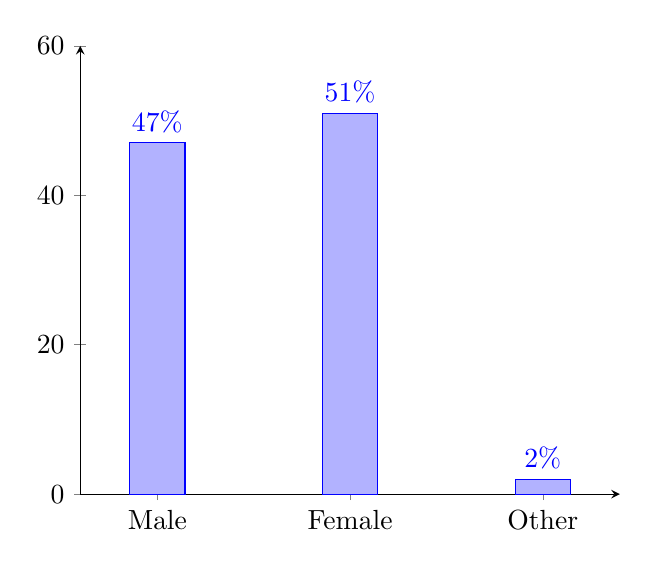
\begin{tikzpicture}
            \begin{axis}[
                ybar,
                bar width=20pt,
                ymin=0,
                ymax=60,
                symbolic x coords={Male,Female,Other},
                xtick=data,
                axis x line=bottom,
                axis y line=left,
                enlarge x limits=0.2,
                nodes near coords={\pgfmathprintnumber\pgfplotspointmeta\%}
            ]
                \addplot coordinates {(Male,47) (Female,51) (Other,2)};
            \end{axis}
        \end{tikzpicture}
        \caption{Genre distribution of participants.}
        \label{fig:genre}
    \end{center}
\end{figure}

\begin{figure}[H]
    \begin{center}
        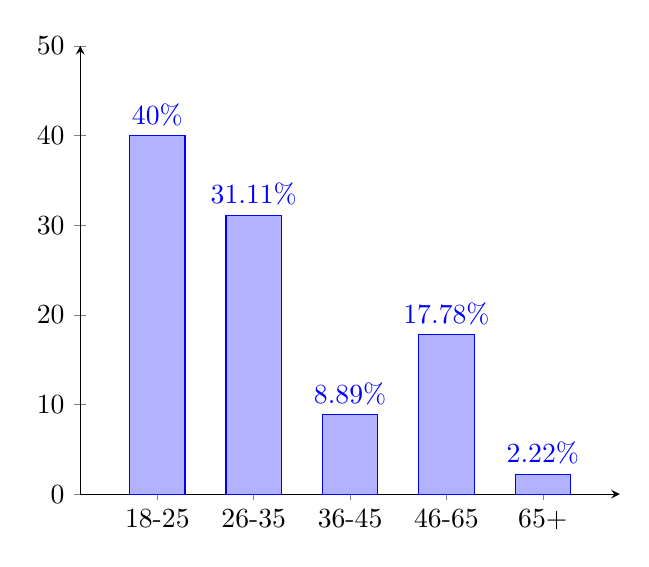
\begin{tikzpicture}
            \begin{axis}[
                ybar,
                bar width=20pt,
                ymin=0,
                ymax=50,
                symbolic x coords={18-25,26-35,36-45,46-65,65+},
                xtick=data,
                axis x line=bottom,
                axis y line=left,
                enlarge x limits=0.2,
                nodes near coords={\pgfmathprintnumber\pgfplotspointmeta\%}
            ]
                \addplot coordinates {(18-25,40) (26-35,31.11) (36-45,8.89) (46-65,17.78) (65+,2.22)};
            \end{axis}
        \end{tikzpicture}
        \caption{Age ranges of participants.}
        \label{fig:age}
    \end{center}
\end{figure}

Most of the respondents have a bachelor's degree, 66.67\% to be exact, 17.78\% have
only finished high school, 2.22\% only have a basic education, 11.11\%
have a master's degree and 2.22\% have a doctorate, as pictured on Figure \ref{fig:education}.

\begin{figure}[H]
    \begin{center}
        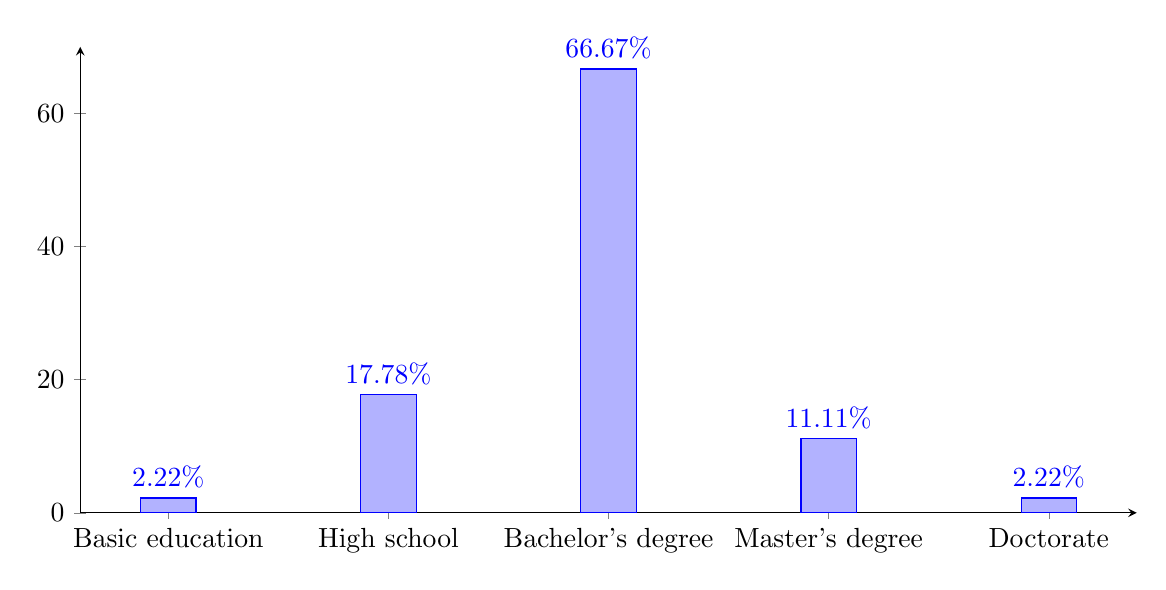
\begin{tikzpicture}
            \begin{axis}[
                height=7.5cm,
                width=15cm,
                ybar,
                bar width=20pt,
                ymin=0,
                ymax=70,
                symbolic x coords={Basic education,High school,Bachelor's degree,Master's degree,Doctorate},
                xtick=data,
                axis x line=bottom,
                axis y line=left,
                enlarge x limits=0.1,
                nodes near coords={\pgfmathprintnumber\pgfplotspointmeta\%}
            ]
                \addplot coordinates {(Basic education,2.22) (High school,17.78) (Bachelor's degree,66.67) (Master's degree,11.11) (Doctorate,2.22)};
            \end{axis}
        \end{tikzpicture}
        \caption{Education qualifications distribution of participants.}
        \label{fig:education}
    \end{center}
\end{figure}

\subsection{Stage 2: An application of theory into practice}
\label{subsection:stage2}

This work proposes an application that gives users information about IoT
devices that inhabit their surroundings, like the type of information these devices
collect and what privacy options are available. This application is developed
for mobile phones due to the fact that these are the most used devices
and people take them everywhere they go, this is important because the application
uses georeferencing to show the location of the IoT devices. This application
has two main objectives, the first is to inform and educate users in order improve
their digital literacy on this particular field (privacy on IoT systems, and
IoT in general) and the other being to give users a way to make informed decisions
to protect their private data, in a concise and convenient place. Generally
the application will show the geolocation of the IoT devices, what type of
device it is, what type of data is being collect by the device. The application
will not detect the devices by itself, this will be done by the users themselves,
in the first iterations of the application it was discussed that the application
itself would automatically detect the devices by using some kind of sniffer
and would categorize what type of device it was and what type of data it
was collecting but it was discovered that this approach was too complex and
so it was not feasible to do with the constraints of this thesis. The application
is developed with Flutter, other options considered were React Native or a
progressive web application, but Flutter uses ahead of time and just in time
compilation, with Dart as it is programming language, while React Native uses
the Javascript programming language that was never created for mobile programming,
so it uses a bridge to convert Javascript to native components for Android
or iOS. Flutter has better performance and as such it was the chosen framework
for this application.

The first step before creating any prototypes or starting the development was
creating a software requirements specification, as can be read on Appendix \ref{appendix:software_requirements},
delineating the scope and vision for the application; the involved stakeholders;
containing contextual, data-flow and swimlane diagrams; software requirements, including
business, technology, functional and non-functional requirements; use cases
and requirements prioritisation.

Users can, when they start the application for the first time, freely use it to see
which devices are in their vicinity,
information about the devices, information about the application itself, and
information about privacy in general and more specifically privacy in IoT systems
which they can use to improve their digital literacy. What they cannot do is
add a new device to the application or edit a device's information. The user has
to create an account first to do these operations. The decision to add an
account creation before the user can add or edit a device is to prevent
bad actors to add bogus data to the application making unusable for the majority
of people, this solution doesn't completely solve this issue (because bad actors
can still create an account and add bogus data anyway) but it helps to slow
down the insertion of bad data.

Upon account creation the only data entry that can be considered sensitive that
the user has to input is an email address.
After the user has created an account and logs in, the user can add devices to the application with the following information:

\begin{itemize}
    \item[$\bullet$]
    The \textbf{name of the device}: This serves to differentiate between the various devices on the application and as such should be unique to each device, it is used on various routes and is one of the first fields that users see about a device. A single device does not have an \textit{official} name, what is more probable is that the device has a model name or is part of a system with it's own name. The user creates the name, this could be abused by bad actors but it is extremely discouraged. It is used for aesthetic reasons.
    \item[$\bullet$]
    The \textbf{category of the device}: This is used to categorize each devices main type of information that the device is collecting. These can be of the following:
    \begin{itemize}
        \item[$\circ$] \textbf{Visual}: The device mainly collects visual information with maybe a video camera.
        \item[$\circ$] \textbf{Audio}: The device mainly collects audio information with a sound recorder.
        \item[$\circ$] \textbf{Presence}: The device can detect the presence of nearby objects or persons. This is not the same as the location category because the device does not know the location of an individual, it merely knows that the individual is nearby. These type of devices can be used, for example, to collect information about how many people frequent a specific store.
        \item[$\circ$] \textbf{Location}: The device can detect the exact or approximate location of an individual, it can use GPS to get this kind of information.
        \item[$\circ$] \textbf{Biometrics}: The devices collects biometric data, this can be the number of steps an individual (or animal) takes, or health related data like the heart beat.
        \item[$\circ$] \textbf{Environment}: These type of devices collect environmental data, they can be used for agriculture or weather forecasting by collecting, for example, temperature, humidity or wind speed/direction data.
        \item[$\circ$] \textbf{Unique identification}: This category is for a device that can uniquely identify an individual, the device itself most likely is not capable of doing it but with other information that the device has access to, it can be used to cross reference of information and as such uniquely identify a person. An example of this would be a device a device that can collect visual data and with facial recognition used against other data in a database it can uniquely identify an individual.
    \end{itemize}
    \item[$\bullet$]
    The \textbf{purpose for the data collection}: Defines what is the purpose for the collection of the data, if a device collects temperature and humidity data and is used by a weather based company or government agency then the purpose for the data collection is for weather forecasting.
    \item[$\bullet$]
    \textbf{Who has access to the collected data}: Disclose an individual or group of individuals that have access to the data of the device, if the device is part of a closed system it can be that only an individual as access to the data but most likely various groups of people have access to the data, some with more data than others depending on the permissions they have. If the device publicizes its data then everyone has access to it.
    \item[$\bullet$]
    \textbf{For how long is the data stored}: Pinpoint the duration of the stored data in the device or system, due to legislation passed in various countries this duration has a limit, in some cases the data cannot be stored for more than one year.
    \item[$\bullet$]
    \textbf{Can the data identify anyone}: Used to quickly identify if a particular device can identify an individual or not. If the device belongs to the "Unique identification" category then this should be active.
    \item[$\bullet$]
    \textbf{What is being done with the data}: This could be assumed to be similar to the \textbf{purpose} field mentioned above but it should be used to diagnose what is being done now with the data collected, in certain situations it might coincide with the purpose for the data collection.
    \item[$\bullet$]
    \textbf{Privacy options}: The user can insert an url for the device's privacy options, in some cases the device, or company, has a website with information on privacy options, or privacy policy. If the device uses a mobile application then a link to the this application can be inserted here.
    \item[$\bullet$]
    \textbf{Coordinates of the device}: Used to express the latitude and longitude of the device so that it can be shown on the map, on the homepage of the application.
    \item[$\bullet$]
    \textbf{Who owns the device}: Who is the device owner, if it belongs to an organization then the name of the organization should appear here otherwise if the device belongs to a person then the person's name should \textbf{not} appear, it should say private or something similar.
\end{itemize}

The user is not required to provide information to satisfy all items on this list, the
only information that is required in order to add a device to the application is
the name, category and coordinates of the device, all other
information is optional but should be provided for the sake of guaranteeing a good
experience to other users of the application. The information provided
should be verified by the user beforehand so that bogus data does not clutter
the application, in this case there are no absolute ways of guaranteeing this
but the maintainer of the application edit wrong information or in some
cases remove it, other users can also edit any device data. This is an
open platform so it is expected that users act in good faith.

% Types of data:
% Health
% Visual
% Audio
% Presence (if user is nearby)
% Location (precise location of user)
% Biometrics
% Environment
% Unique identification (with the help of other means)

% Information to be added to the app:
% What is the purpose of the data collection
% Who can access the data
% For how long is it stored
% Can the data identify anyone
% What is done with this data

% \section{Current Stage of the Work}

% The preliminary results of the study, based on 10 responses, show that everyone
% agrees that privacy is important to them and some people know that they
% should not share their personal information with anyone they do not trust
% (like clicking on random urls or using unprotected websites/software), but
% most of them think that privacy and security are the same concept, most
% respondents also do not read privacy notices but accept them to access the
% information they want to get to, most respondents use their devices mostly
% to access social networks and for work, when it comes to IoT, there is a
% dissonance between knowing the term and using devices like smart watches
% or RFID enabled devices, from the respondents that answered yes to using
% IoT devices most use because of work. It is also noted that most respondent
% have a background in engineering, so the responses are skewed. As a result,
% the survey will remain open to gather a larger number of responses and participants
% for more significant results and generalizations.

% \begin{table}[ht]
% \centering
% \begin{adjustbox}{width=0.5\textwidth}
% \small
% \noindent\begin{tabular}{p{0.17\textwidth}*{20}{|p{0.01\textwidth}}|}
% \hline
% \multicolumn{0}{|c|}{Work plan}
%     & \multicolumn{4}{c|}{January}
%     & \multicolumn{4}{c|}{February}
%     & \multicolumn{4}{c|}{March}
%     & \multicolumn{4}{c|}{April}
%     & \multicolumn{4}{c|}{May}
%     \\
% \hline
% \hline
% \multicolumn{0}{|l|}{Week}
%     & 1 & 2 & 3 & 4 & 1 & 2 & 3 & 4& 1 & 2 & 3 & 4& 1 & 2 & 3 & 4& 1 & 2 & 3 & 4 \\
% \hline
% % using the on macro to fill in twenty cells as `on'
% \multicolumn{0}{|l|}{Discovery and planning}
%     & \cellcolor[cmyk]{1,1,0,0}&&&& &&&& &&&& &&&&&&& \\
% \hline
% \multicolumn{0}{|l|}{Research enquiry}
%     & \cellcolor[cmyk]{1,1,0,0} & \cellcolor[cmyk]{1,1,0,0} & \cellcolor[cmyk]{1,1,0,0} & \cellcolor[cmyk]{1,1,0,0} & \cellcolor[cmyk]{1,1,0,0} & \cellcolor[cmyk]{1,1,0,0} & \cellcolor[cmyk]{1,1,0,0} & \cellcolor[cmyk]{1,1,0,0} & \cellcolor[cmyk]{1,1,0,0} & \cellcolor[cmyk]{1,1,0,0} & \cellcolor[cmyk]{1,1,0,0} & \cellcolor[cmyk]{1,1,0,0} &&&& &&&& \\
% \hline
% \multicolumn{0}{|l|}{State of the art}
%     & \cellcolor[cmyk]{1,1,0,0} & \cellcolor[cmyk]{1,1,0,0} & \cellcolor[cmyk]{1,1,0,0} & \cellcolor[cmyk]{1,1,0,0} & \cellcolor[cmyk]{1,1,0,0} & \cellcolor[cmyk]{1,1,0,0} & \cellcolor[cmyk]{1,1,0,0} & \cellcolor[cmyk]{1,1,0,0} &&&& &&&& &&&& \\
% \hline
% \multicolumn{0}{|l|}{Project requirements}
%     & \cellcolor[cmyk]{1,1,0,0} & \cellcolor[cmyk]{1,1,0,0} & \cellcolor[cmyk]{1,1,0,0} & \cellcolor[cmyk]{1,1,0,0} &&&& &&&& &&&& &&&& \\
% \hline
% \multicolumn{0}{|l|}{Wireframes and user stories}
%     &&&& & \cellcolor[cmyk]{1,1,0,0} & \cellcolor[cmyk]{1,1,0,0} & \cellcolor[cmyk]{1,1,0,0} & \cellcolor[cmyk]{1,1,0,0} &&&& &&&& &&&& \\
% \hline
% \multicolumn{0}{|l|}{Prototyping and refinement}
%     &&&&&& && \cellcolor[cmyk]{1,1,0,0} & \cellcolor[cmyk]{1,1,0,0} & \cellcolor[cmyk]{1,1,0,0} & \cellcolor[cmyk]{1,1,0,0} &&&& &&&& &  \\
% \hline
% \multicolumn{0}{|l|}{Development}
%     &&&& &&&& & \cellcolor[cmyk]{1,1,0,0} & \cellcolor[cmyk]{1,1,0,0} & \cellcolor[cmyk]{1,1,0,0} & \cellcolor[cmyk]{1,1,0,0} & \cellcolor[cmyk]{1,1,0,0} & \cellcolor[cmyk]{1,1,0,0} & \cellcolor[cmyk]{1,1,0,0} & \cellcolor[cmyk]{1,1,0,0} & \cellcolor[cmyk]{1,1,0,0} & \cellcolor[cmyk]{1,1,0,0} & \cellcolor[cmyk]{1,1,0,0} & \cellcolor[cmyk]{1,1,0,0} \\
% \hline
% \multicolumn{0}{|l|}{Tests and iterations}
%     &&&& &&&& &&& & \cellcolor[cmyk]{1,1,0,0} & \cellcolor[cmyk]{1,1,0,0} & \cellcolor[cmyk]{1,1,0,0} & \cellcolor[cmyk]{1,1,0,0} & \cellcolor[cmyk]{1,1,0,0} &&&&  \\
% \hline
% \multicolumn{0}{|l|}{Release and documentation}
%     &&&& &&&& &&&& &&&& & \cellcolor[cmyk]{1,1,0,0} & \cellcolor[cmyk]{1,1,0,0} & \cellcolor[cmyk]{1,1,0,0} & \cellcolor[cmyk]{1,1,0,0} \\
% \hline
% \end{tabular}
% \end{adjustbox}
% \vspace{1em}
% \caption{Work plan timeline}
% \label{workchart}
% \end{table}

% As can be seen in Table \ref{workchart}, the first months will involve the
% design of the application and the enquiry of the study followed by the development
% of the application and the synthesis of the study, and finally testing and
% refinement of the application. Because of the exploratory nature of this
% work the application might suffer alterations to the design, specially in
% the testing stage, and also depending on the results of the study.

\begin{figure}
    \centering
    \begin{subfigure}{0.33\textwidth}
        \centering
        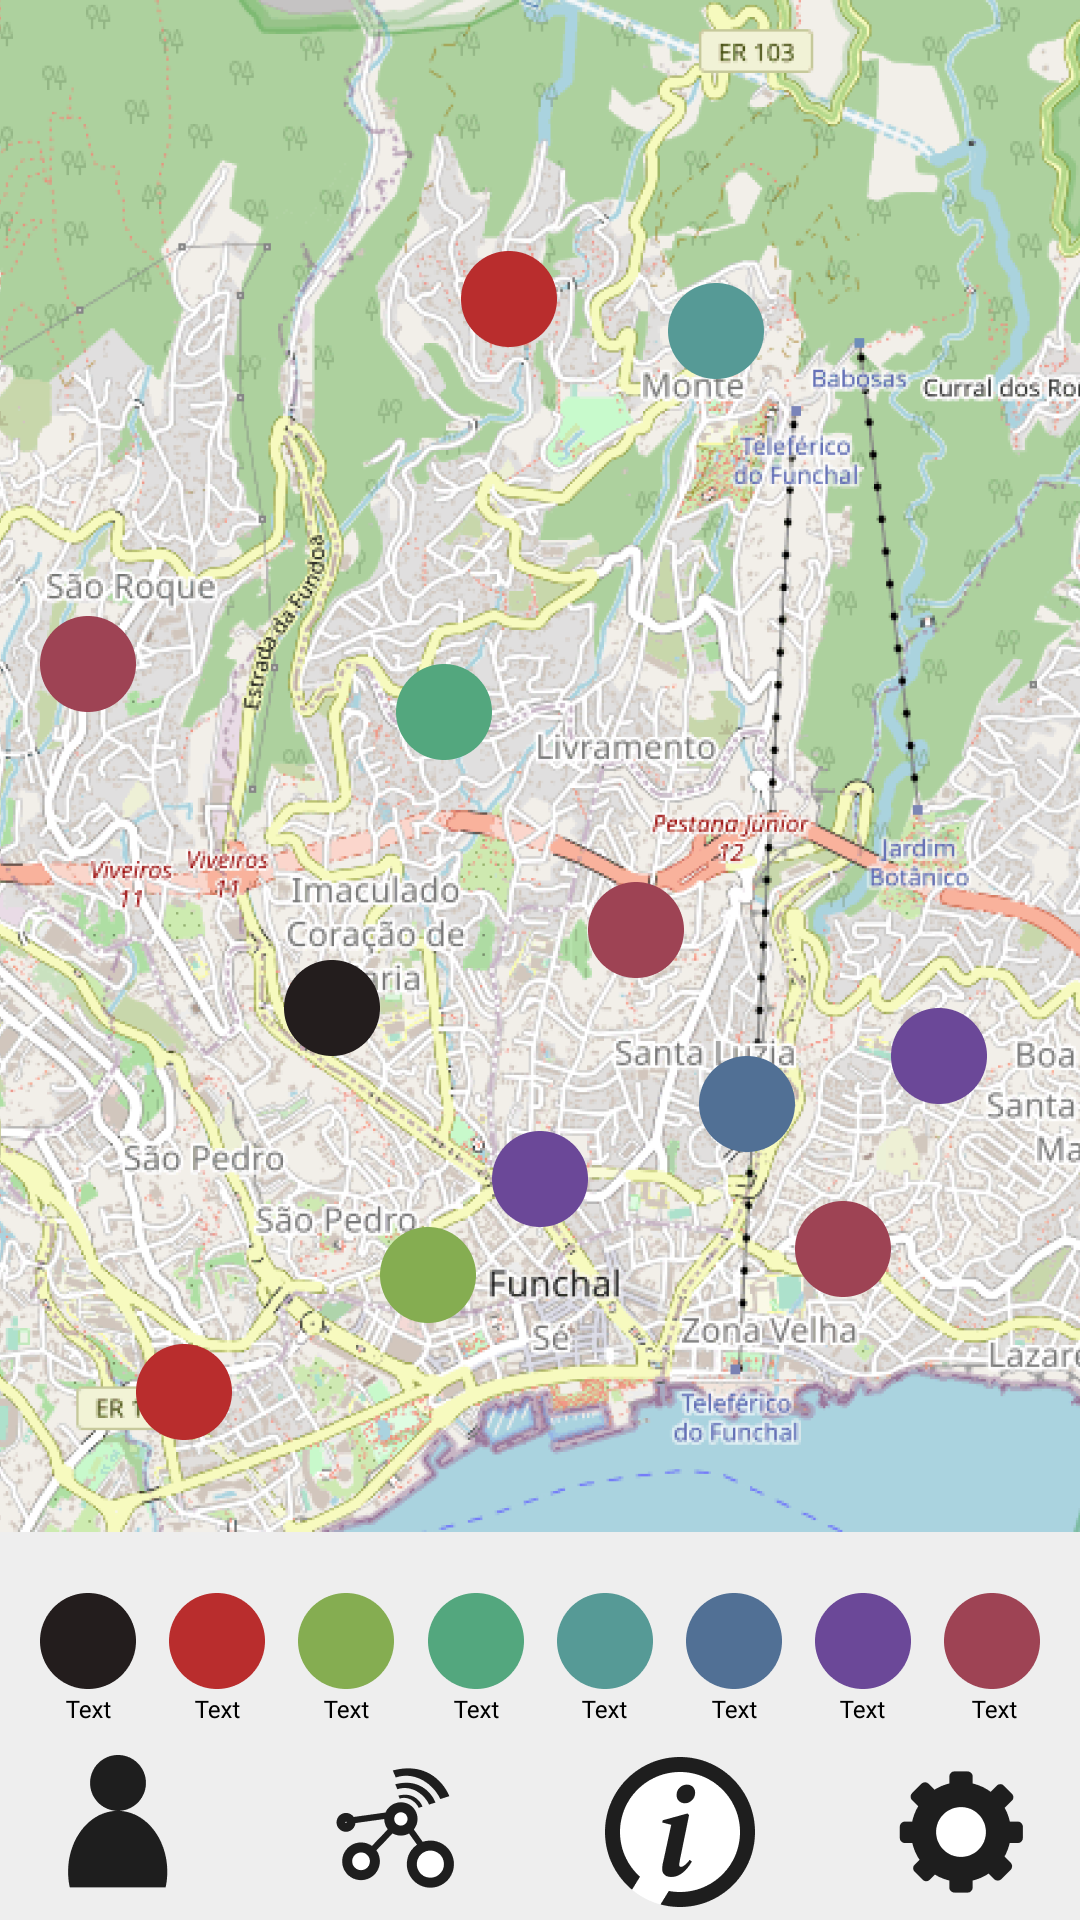
\includegraphics[width=130pt]{../assets/images/low_homepage.png}
        \caption{}
        \label{fig:lowhome}
    \end{subfigure}%
    \begin{subfigure}{0.33\textwidth}
        \centering
        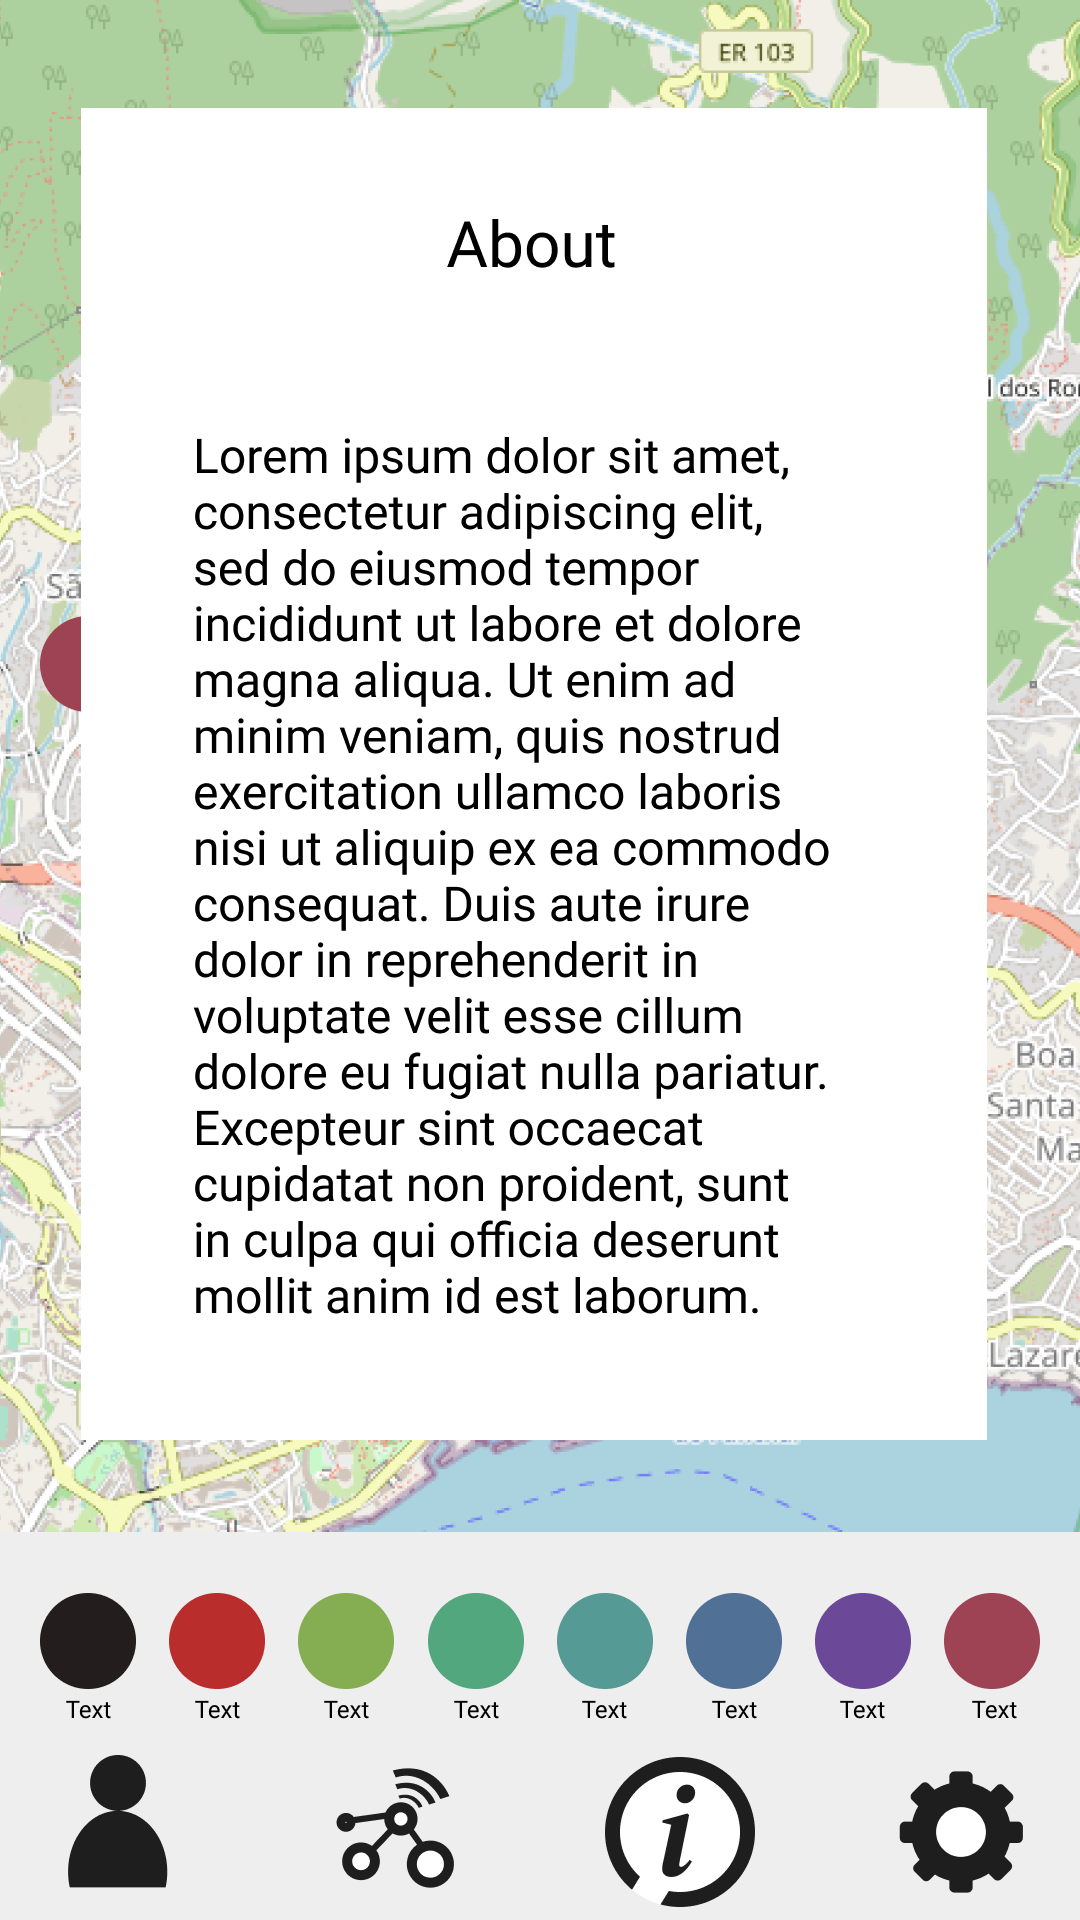
\includegraphics[width=130pt]{../assets/images/low_about.png}
        \caption{}
        \label{fig:lowabout}
    \end{subfigure}%
    \begin{subfigure}{0.33\textwidth}
        \centering
        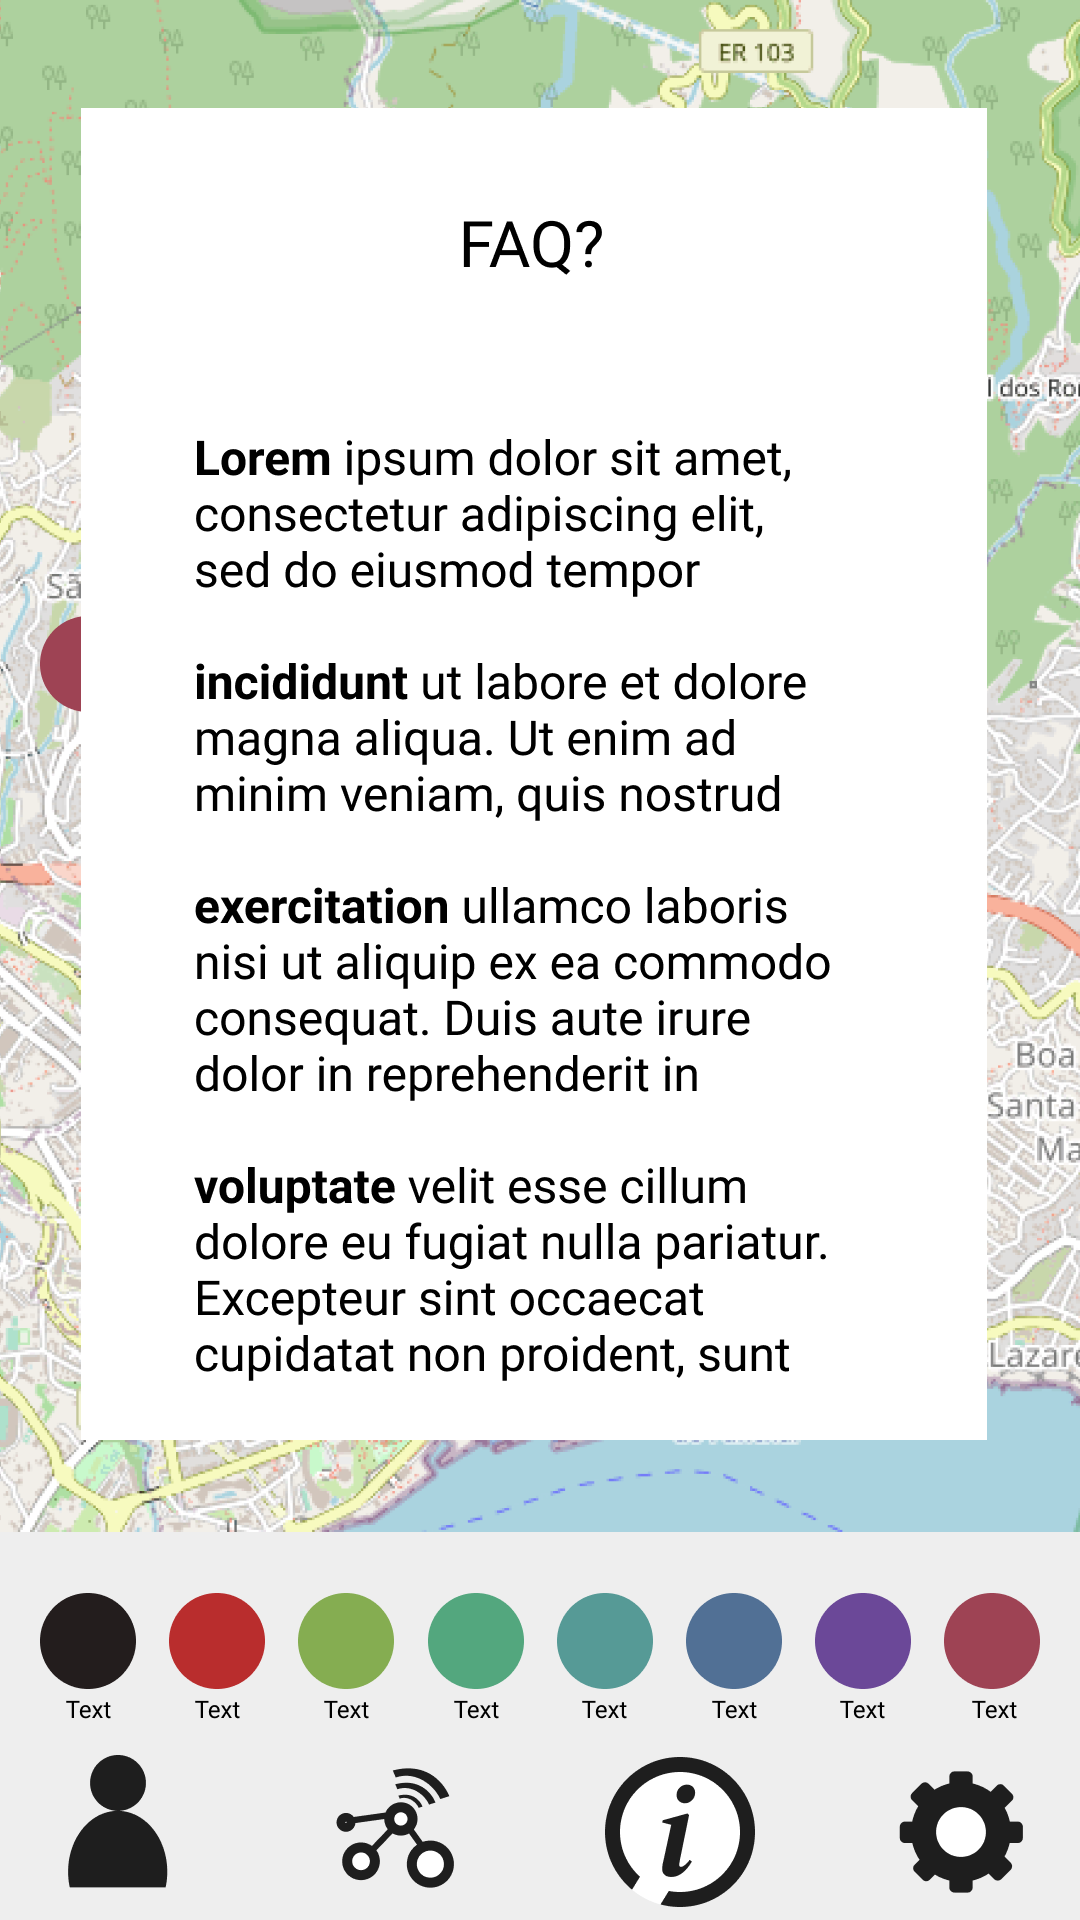
\includegraphics[width=130pt]{../assets/images/low_more_info.png}
        \caption{}
        \label{fig:lowfaq}
    \end{subfigure}%
    \caption{Low level prototype of (a) homepage, (b) about and (c) FAQ pages.}
    \label{fig:lowlevelprototype}
\end{figure}

After creating the software requirements specification, the prototypes were
created. For the creation of the prototypes the following tools were used: Figma
and GIMP.

At first a low level prototype was made in order to understand the
general design and user interaction of the application. Figure \ref{fig:lowlevelprototype}
shows tree pages of the low level prototype, these are the homepage, about
and faq pages, this prototype has a navigation menu on the bottom where the
other pages of the application can be selected along with some information
above the page icons, this information is supposed to be the categories of
the devices, the logic would be that the user could tap one of these categories
and only devices of that category should be displayed on the map. It can
be seen that between the three pages the map stays in the background and
the various pages work like an overlay on the homepage, this would be
changed in subsequent prototype versions.

\begin{figure}
    \centering
    \begin{subfigure}{0.33\textwidth}
        \centering
        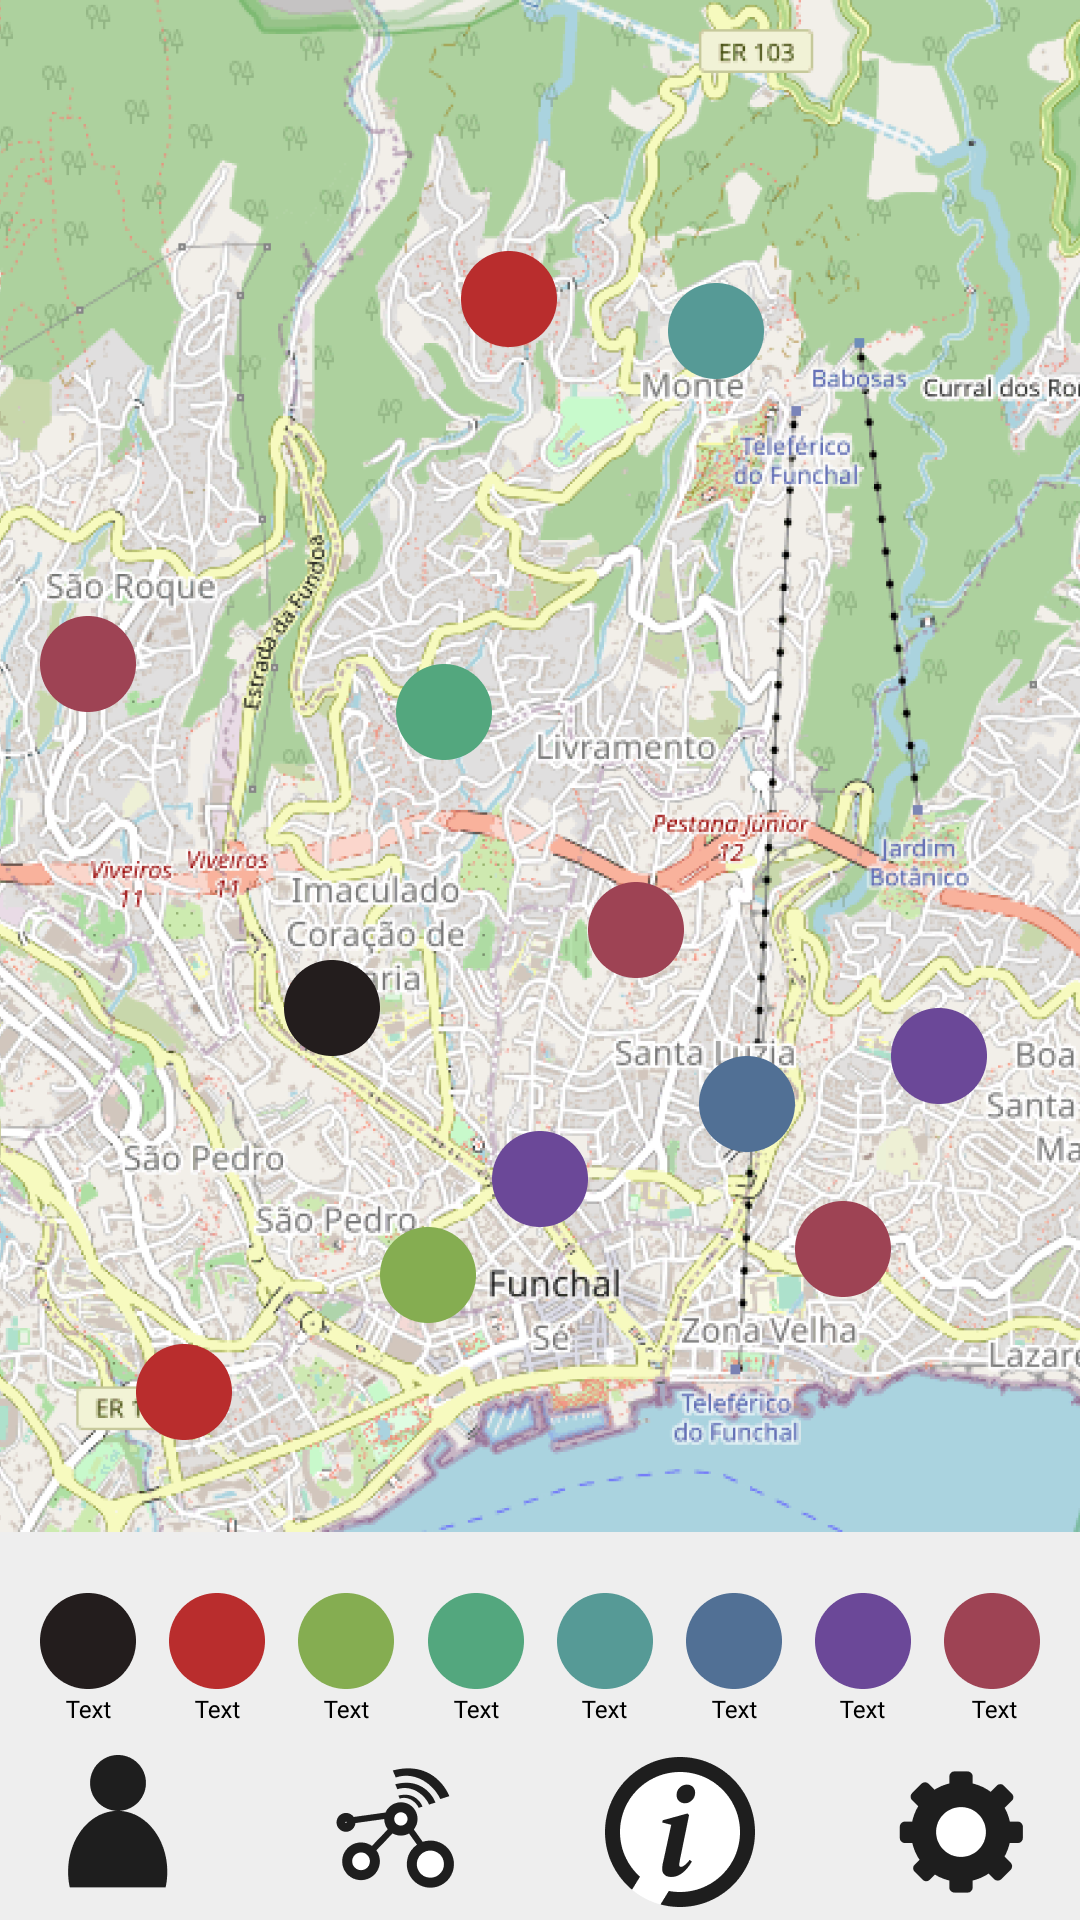
\includegraphics[width=130pt]{../assets/images/low_homepage.png}
        \caption{}
        \label{fig:mediumhome}
    \end{subfigure}%
    \begin{subfigure}{0.33\textwidth}
        \centering
        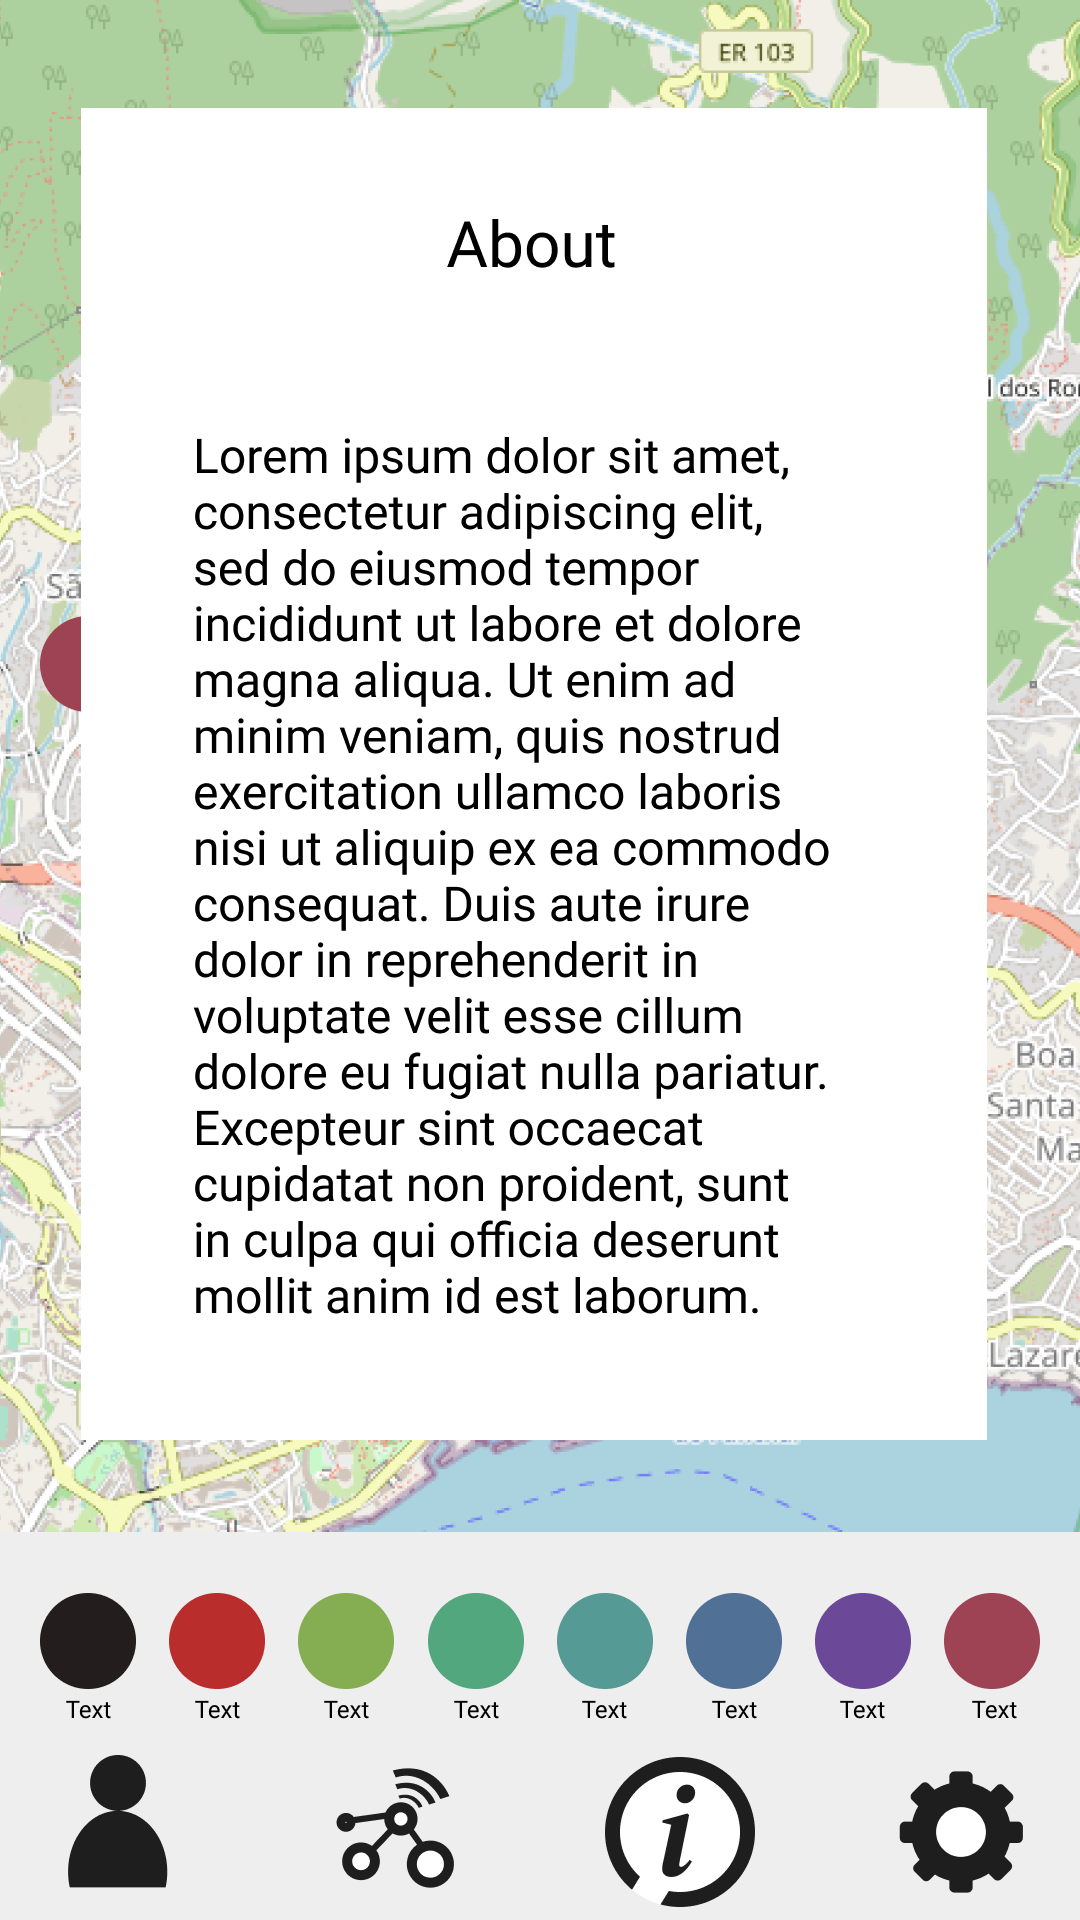
\includegraphics[width=130pt]{../assets/images/low_about.png}
        \caption{}
        \label{fig:mediumabout}
    \end{subfigure}%
    \begin{subfigure}{0.33\textwidth}
        \centering
        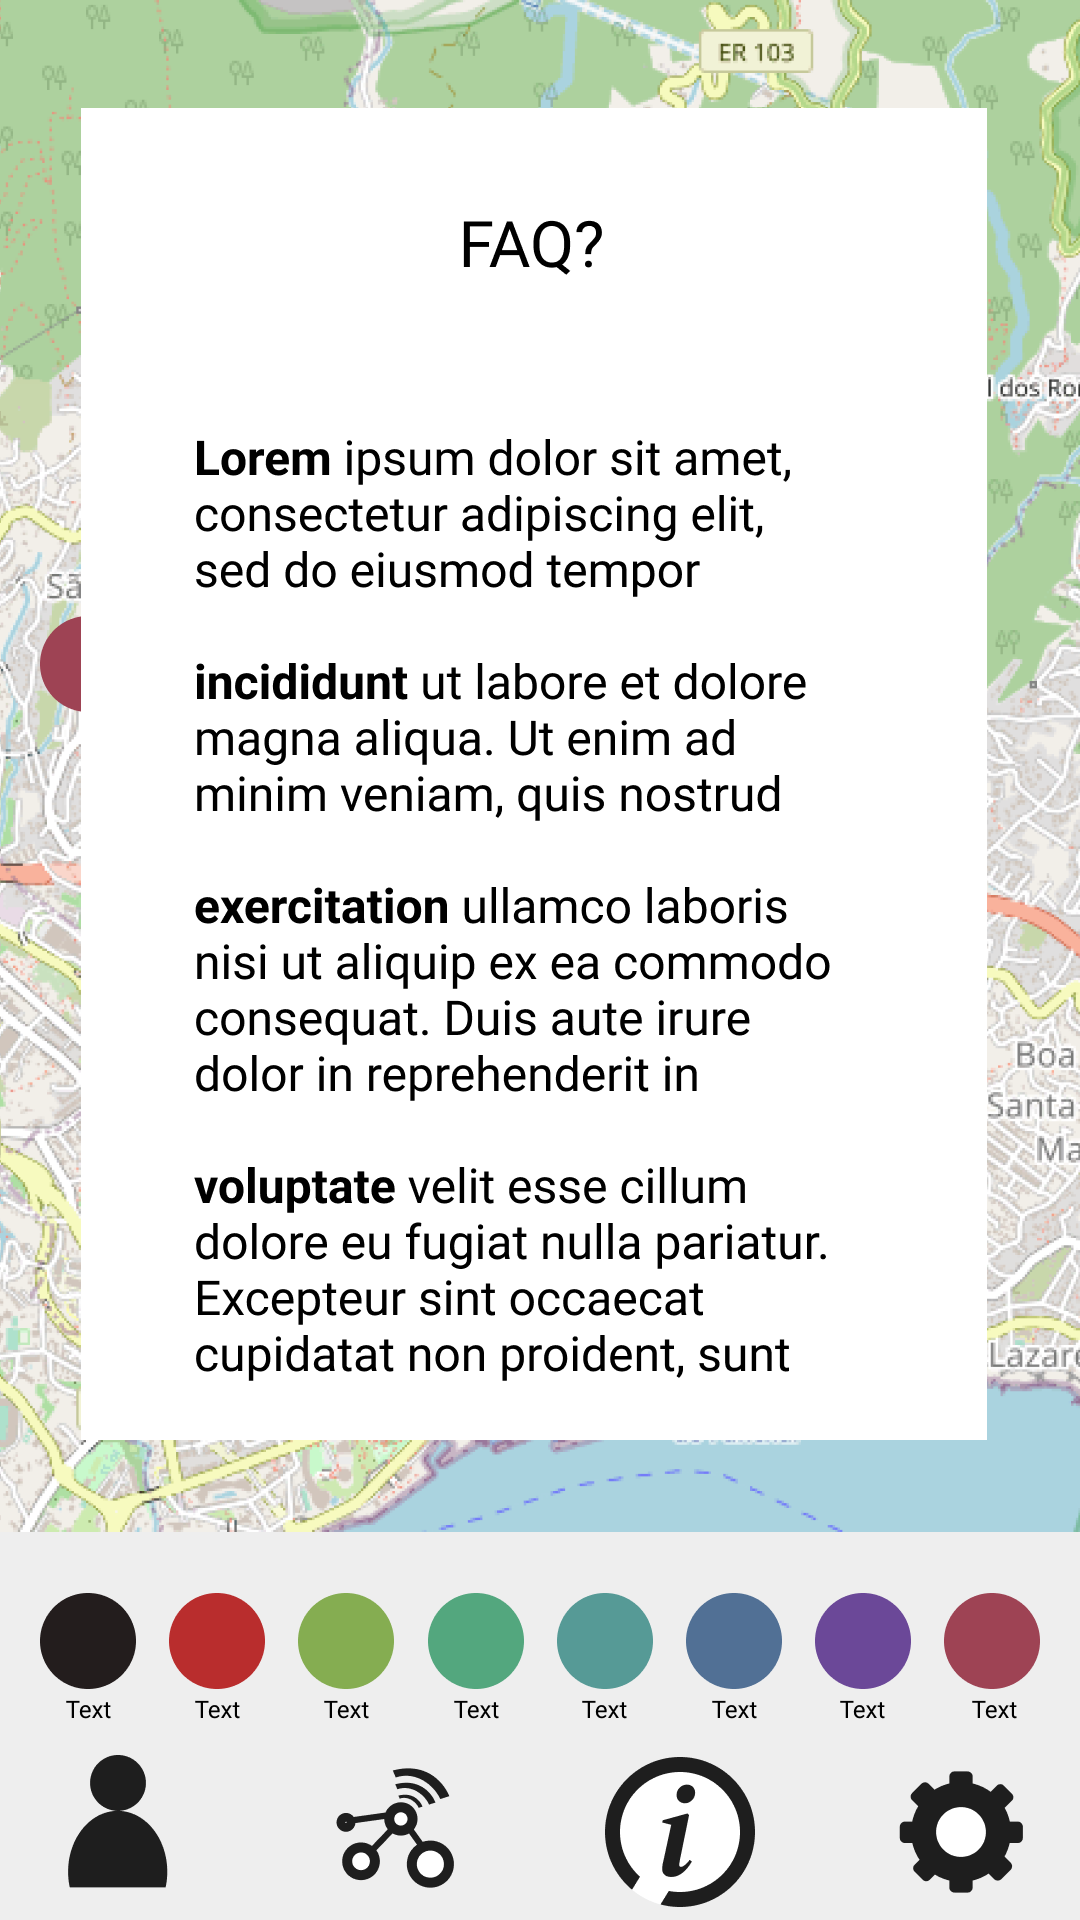
\includegraphics[width=130pt]{../assets/images/low_more_info.png}
        \caption{}
        \label{fig:mediumfaq}
    \end{subfigure}%
    \caption{Medium level prototype of (a) homepage, (b) about and (c) FAQ pages.}
    \label{fig:mediumlevelprototype}
\end{figure}

\begin{figure}[H]
    \centering
    \begin{subfigure}{0.33\textwidth}
        \centering
        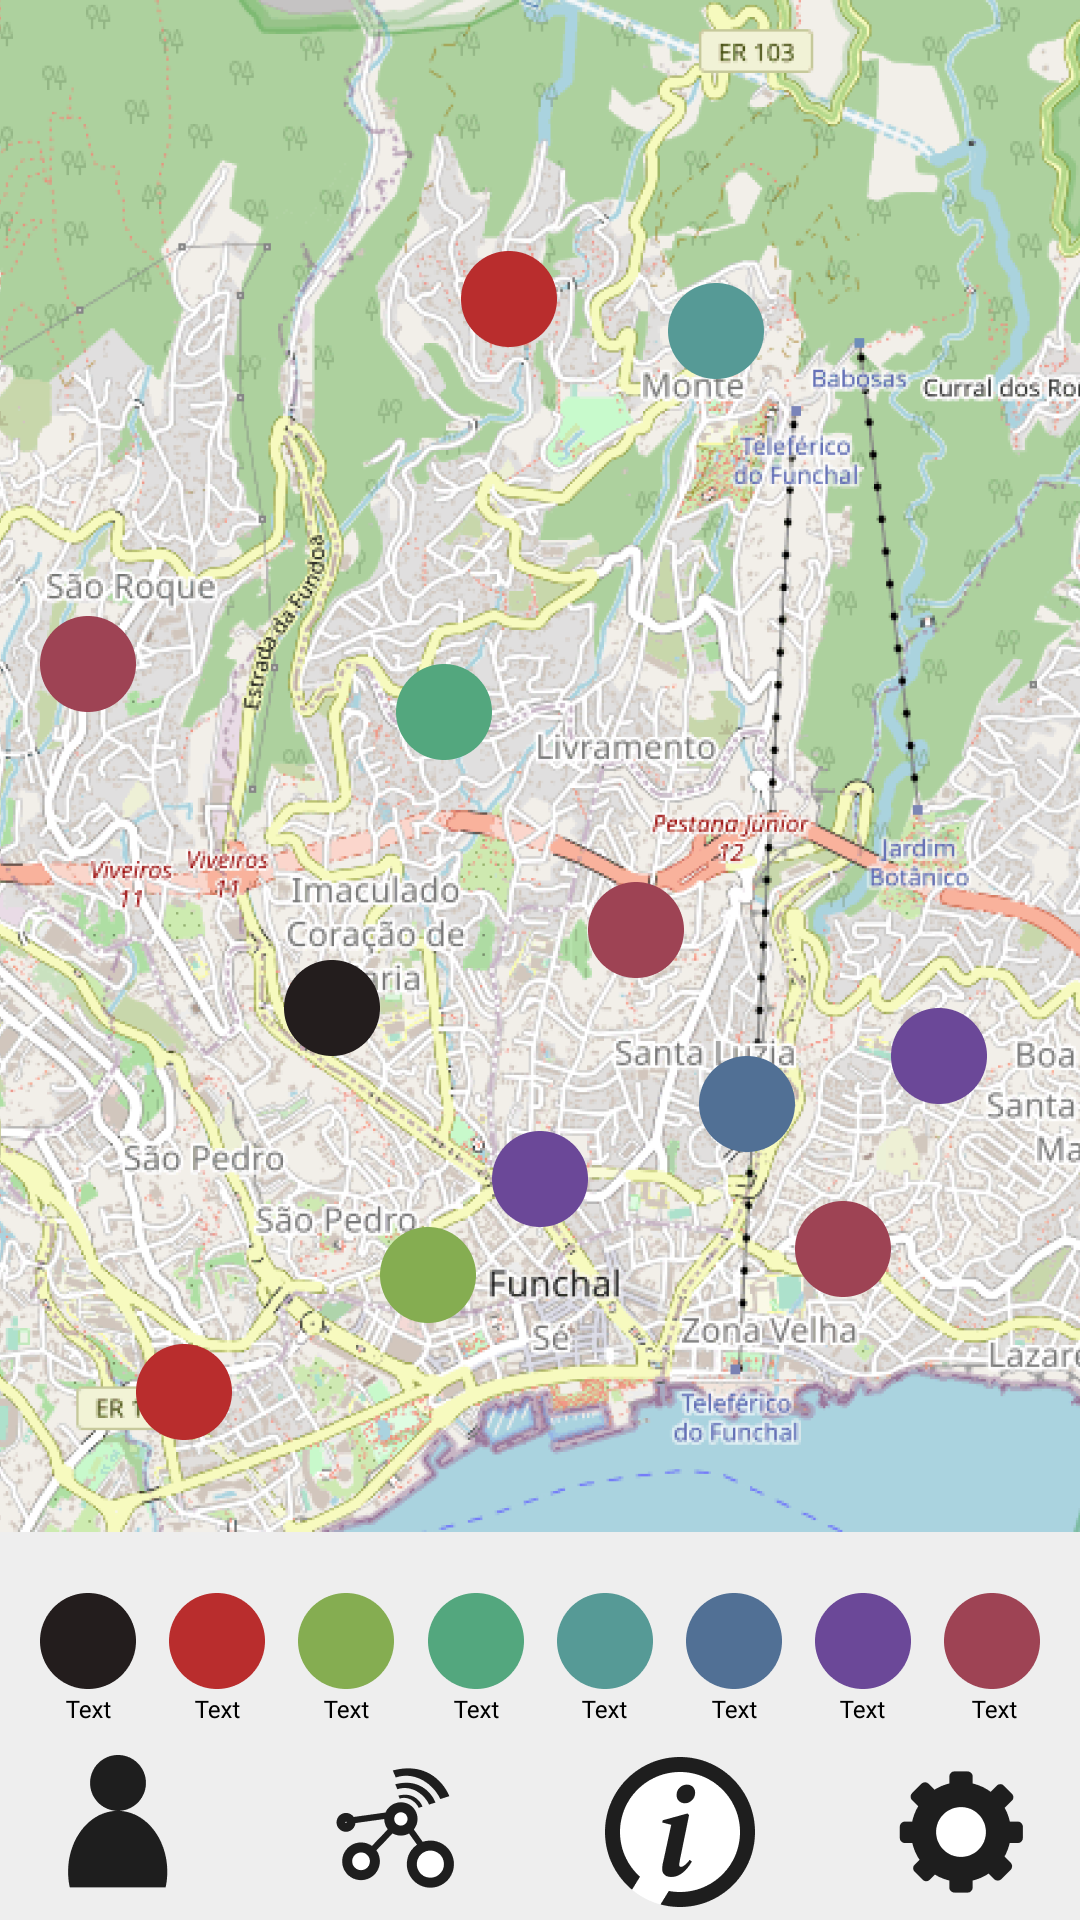
\includegraphics[width=130pt]{../assets/images/low_homepage.png}
        \caption{}
        \label{fig:highhome}
    \end{subfigure}%
    \begin{subfigure}{0.33\textwidth}
        \centering
        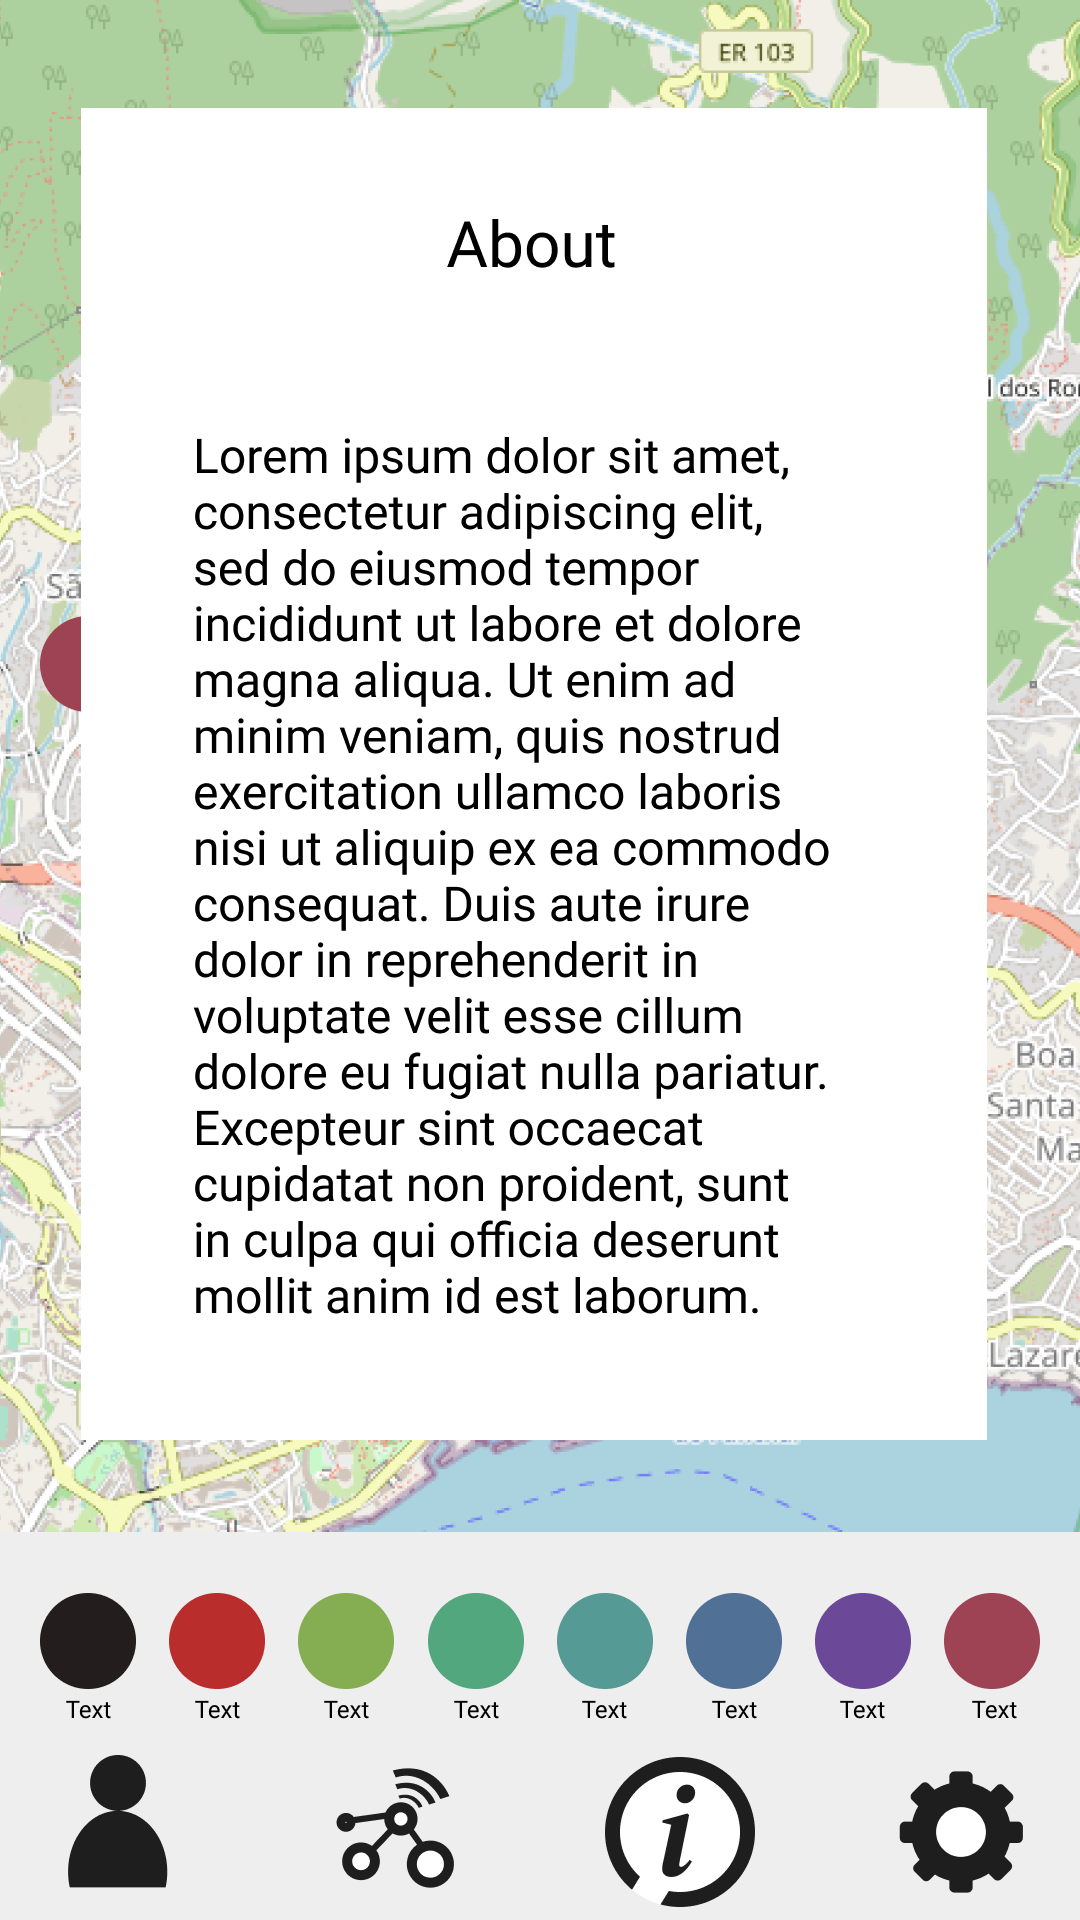
\includegraphics[width=130pt]{../assets/images/low_about.png}
        \caption{}
        \label{fig:highabout}
    \end{subfigure}%
    \begin{subfigure}{0.33\textwidth}
        \centering
        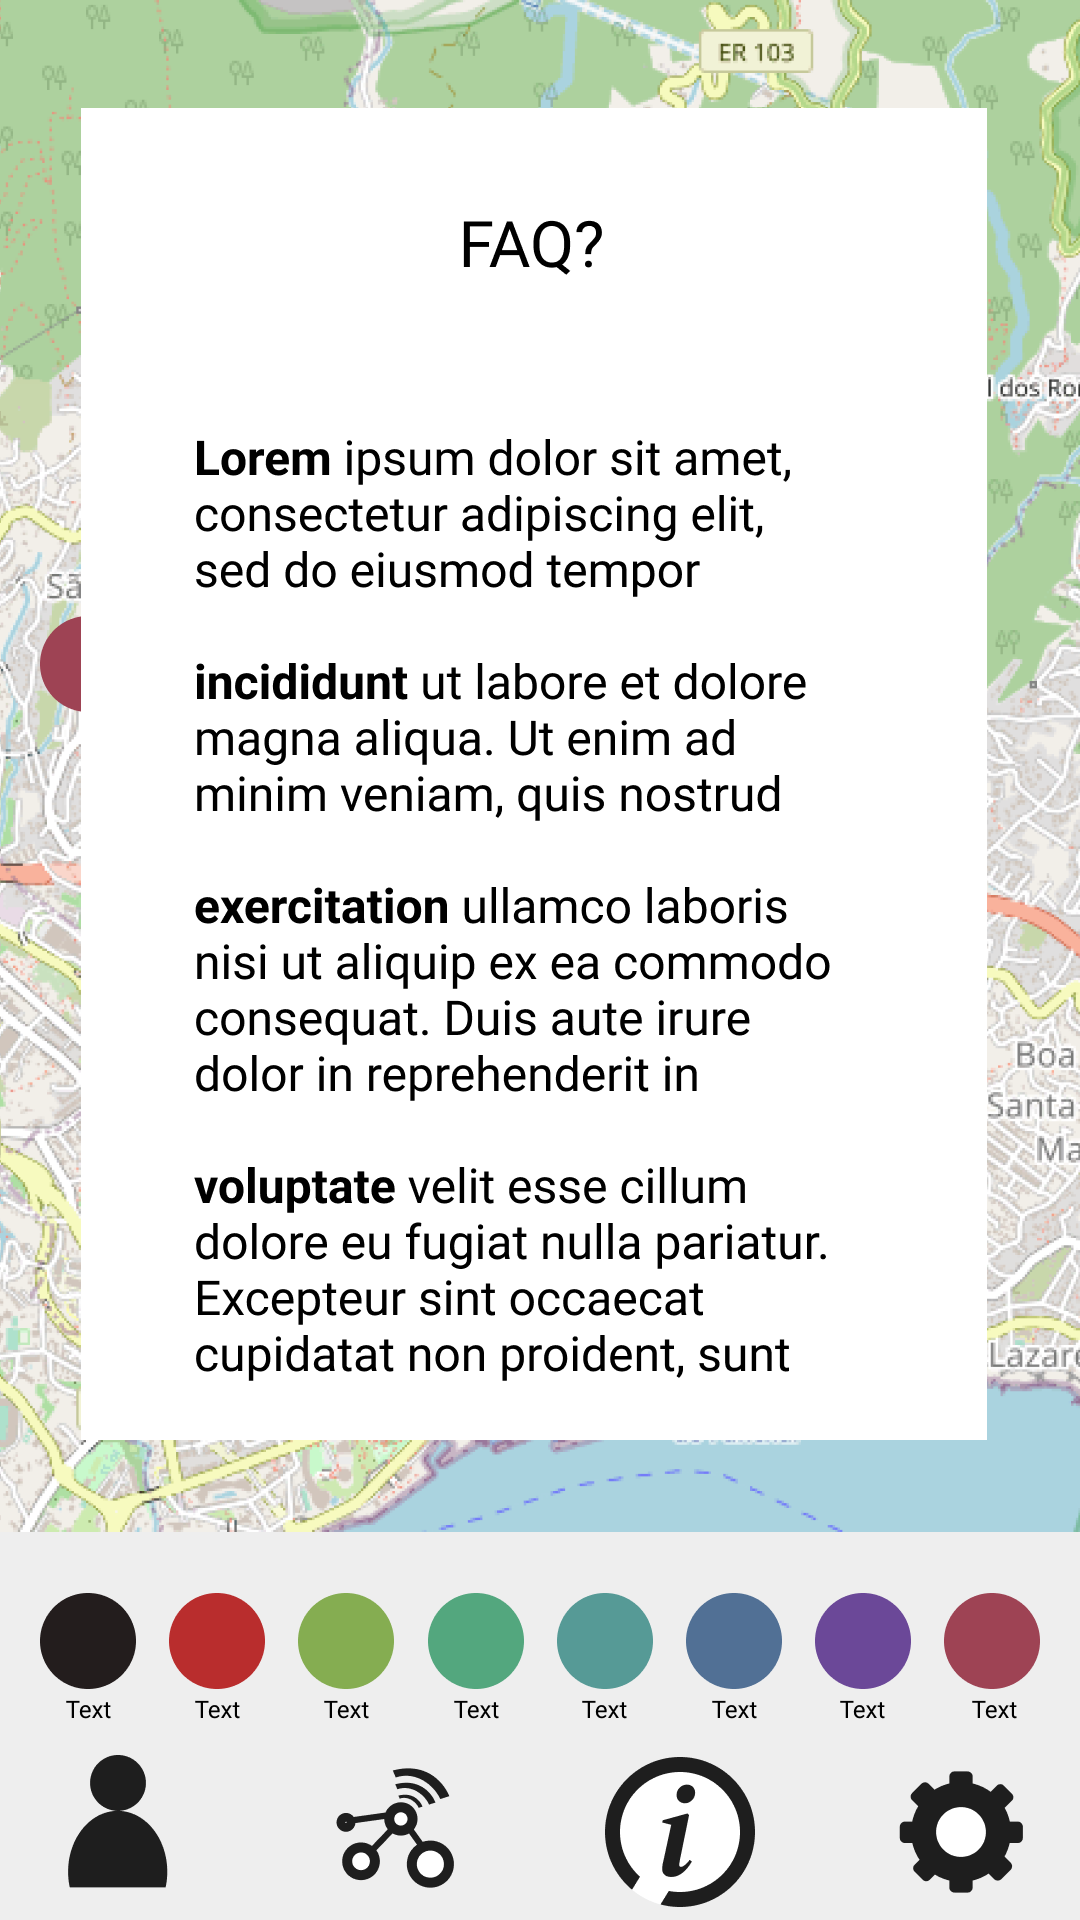
\includegraphics[width=130pt]{../assets/images/low_more_info.png}
        \caption{}
        \label{fig:highfaq}
    \end{subfigure}%
    \caption{High level prototype of (a) homepage, (b) about and (c) FAQ pages.}
    \label{fig:highlevelprototype}
\end{figure}

\begin{figure}[H]
    \centering
    \begin{subfigure}{0.30\textwidth}
        \centering
        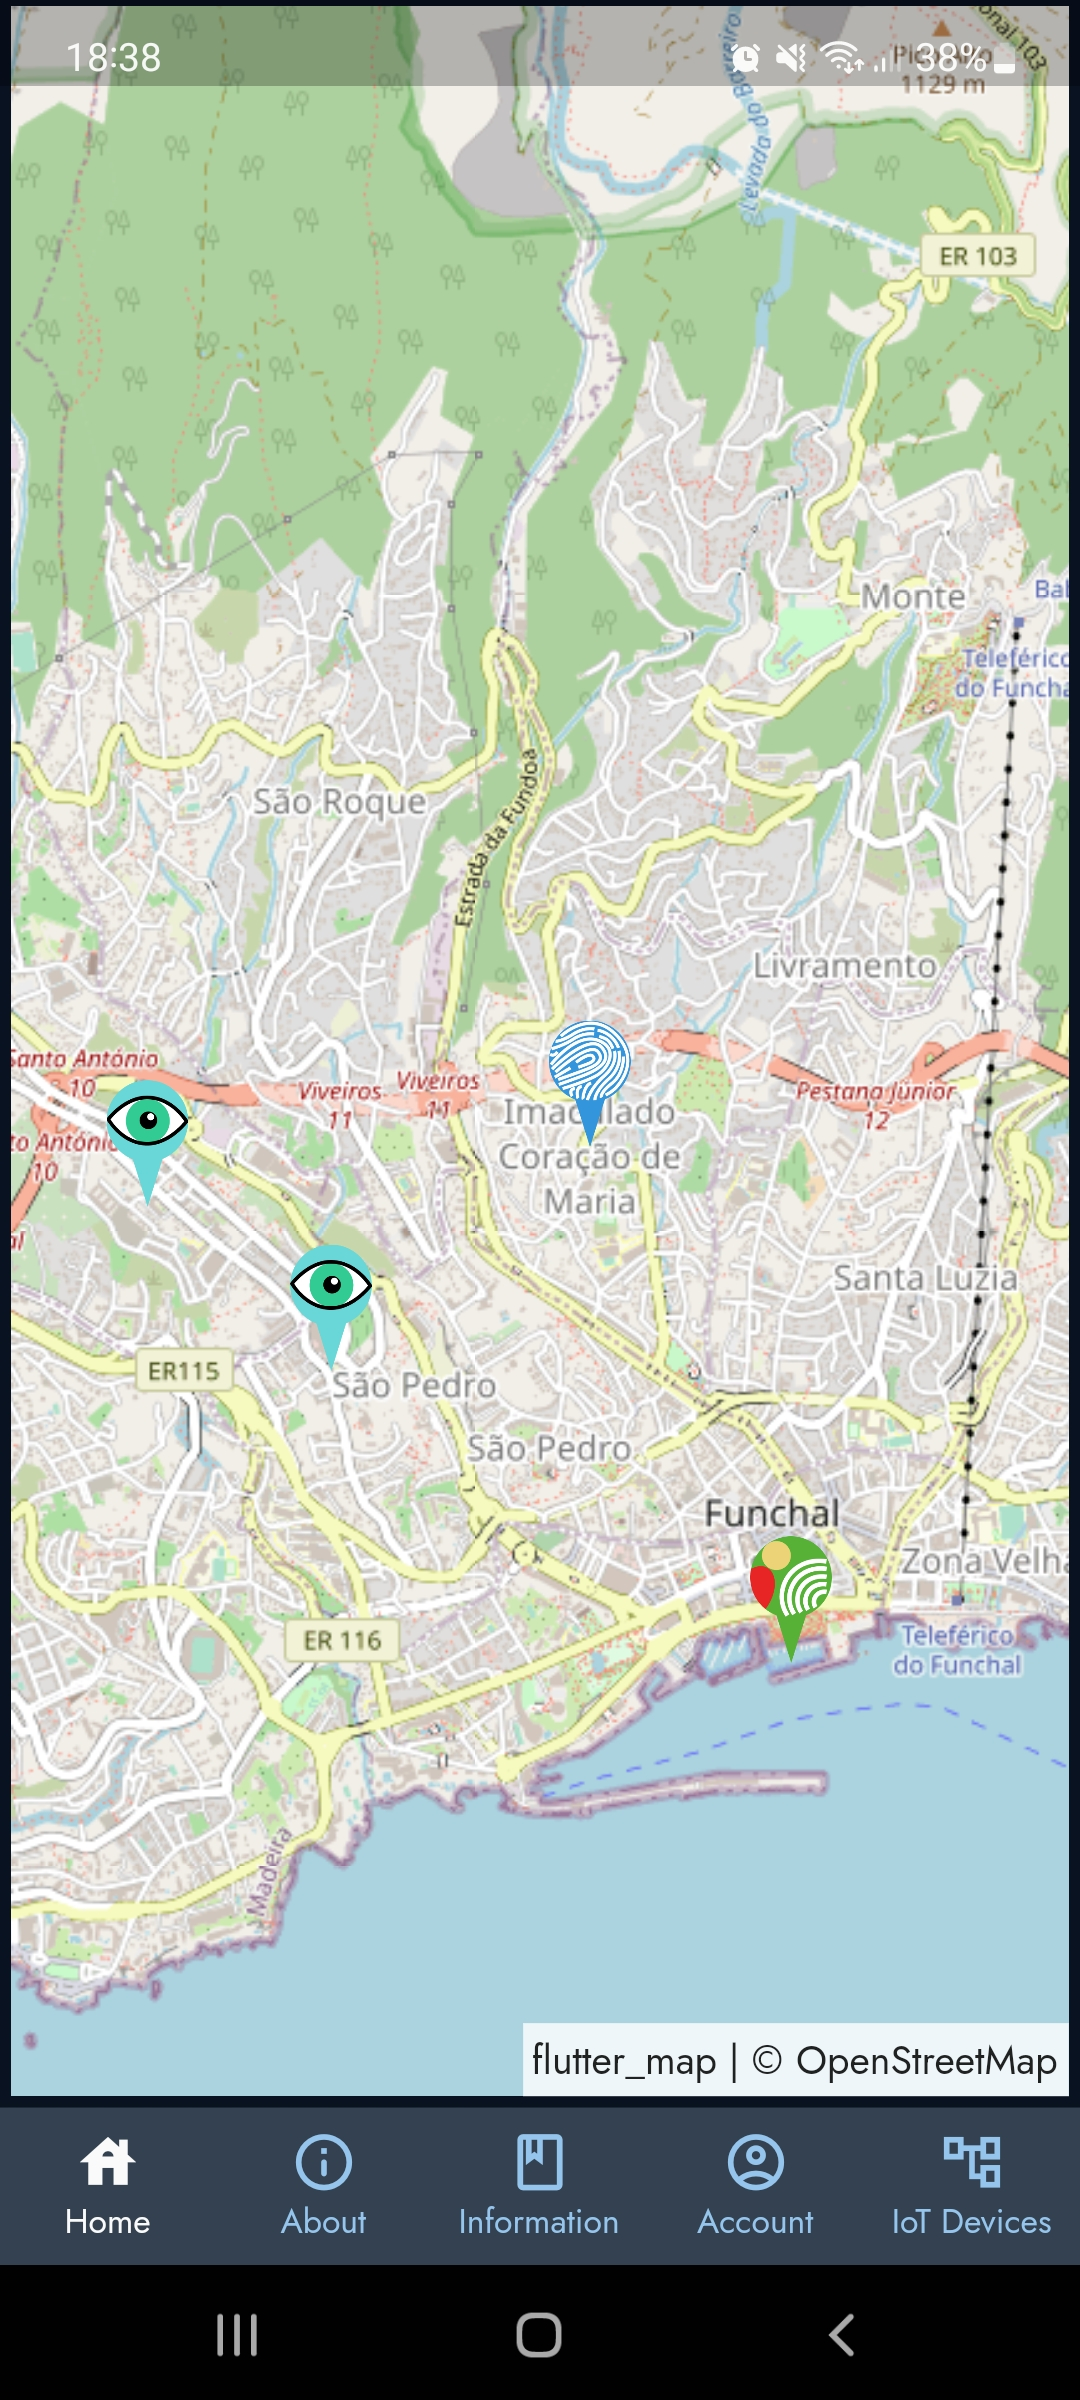
\includegraphics[width=125pt]{../assets/images/live_homepage.jpg}
        \caption{}
        \label{fig:highhome}
    \end{subfigure}
    \begin{subfigure}{0.30\textwidth}
        \centering
        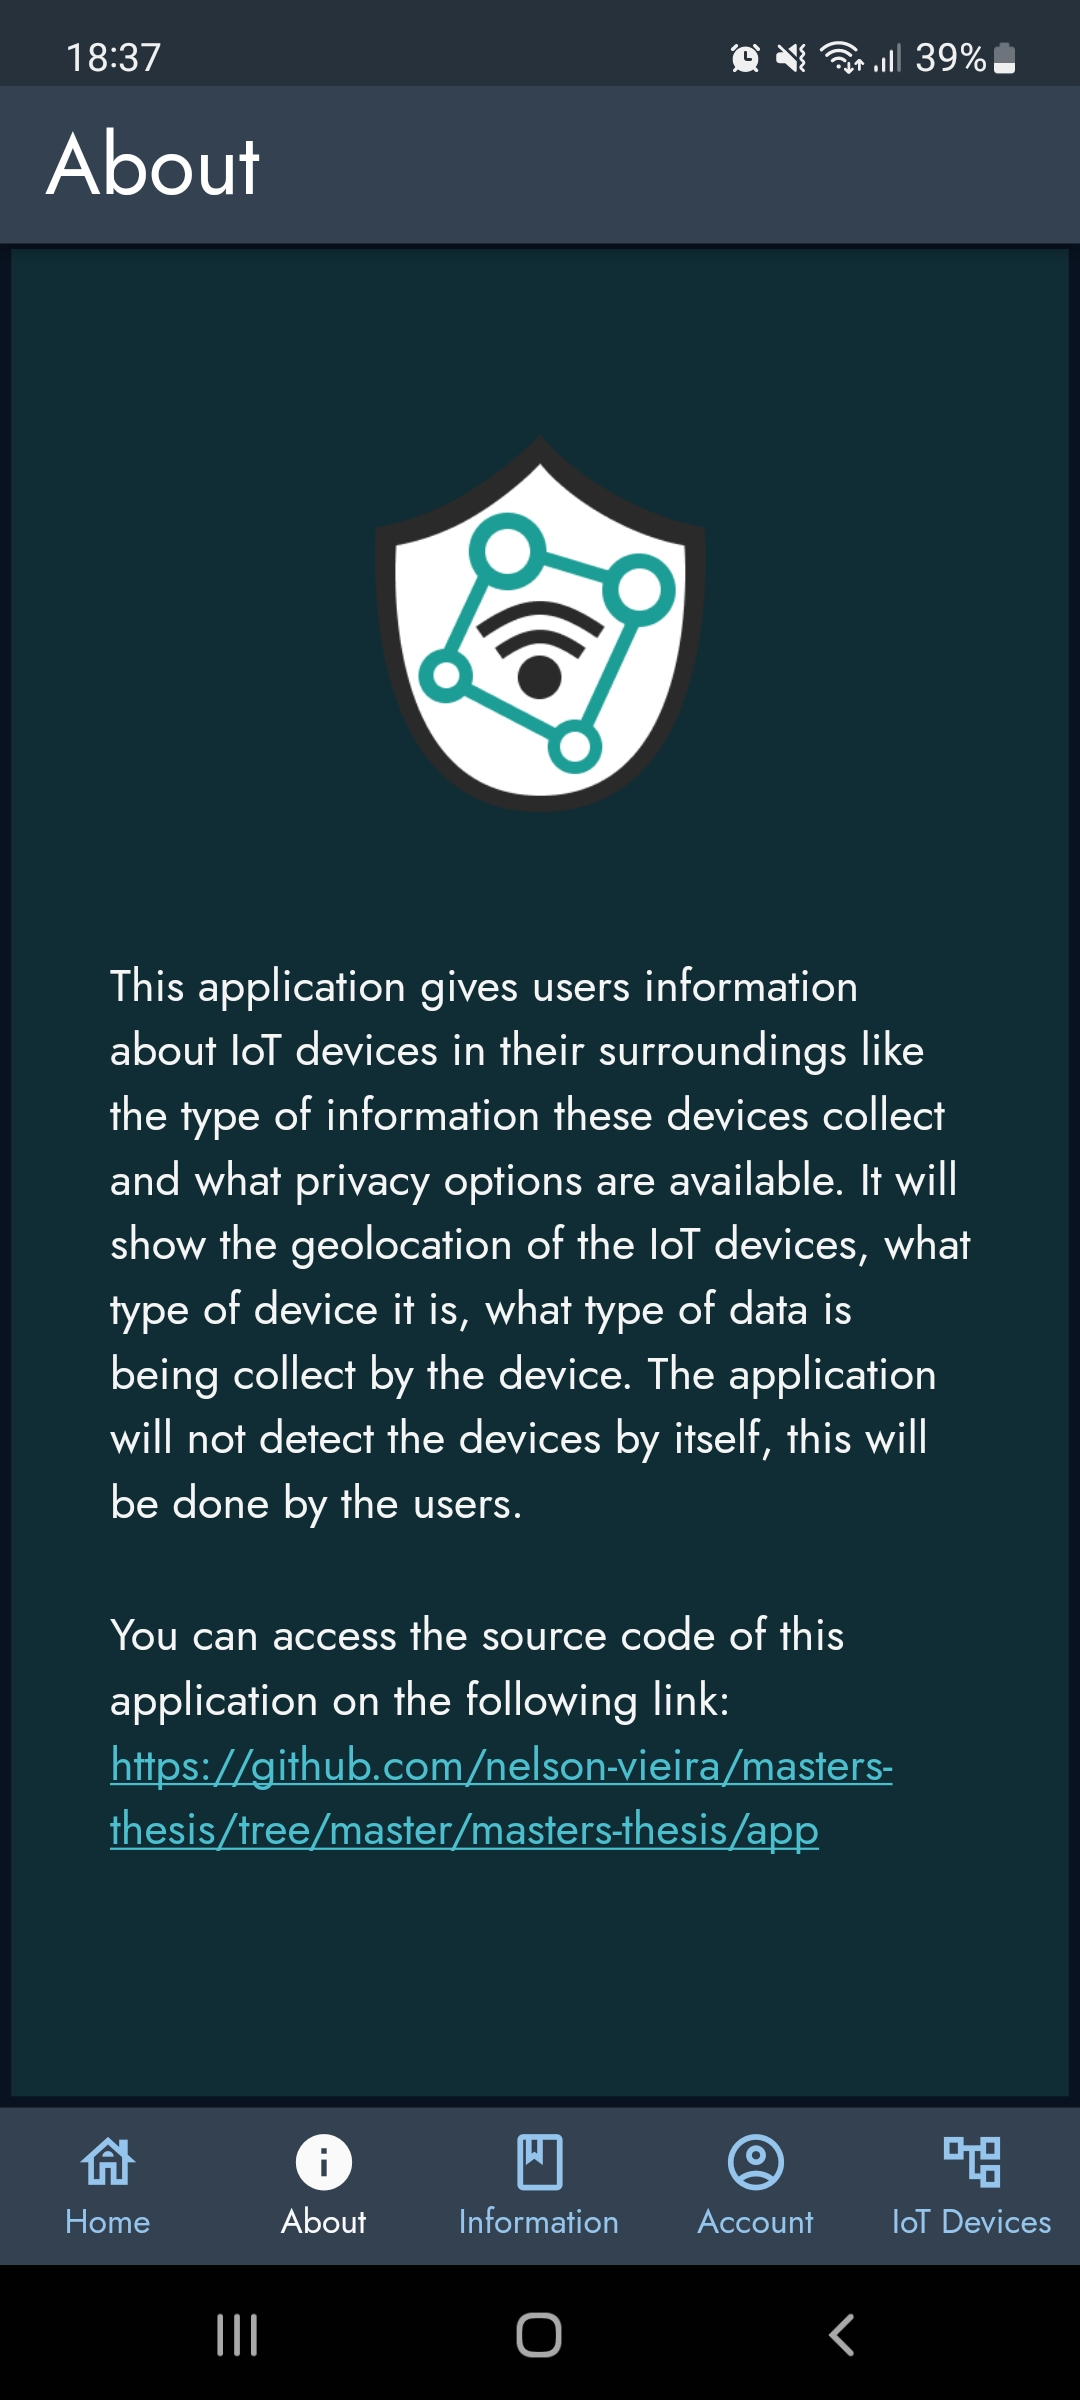
\includegraphics[width=125pt]{../assets/images/live_about.jpg}
        \caption{}
        \label{fig:highabout}
    \end{subfigure}
    \begin{subfigure}{0.30\textwidth}
        \centering
        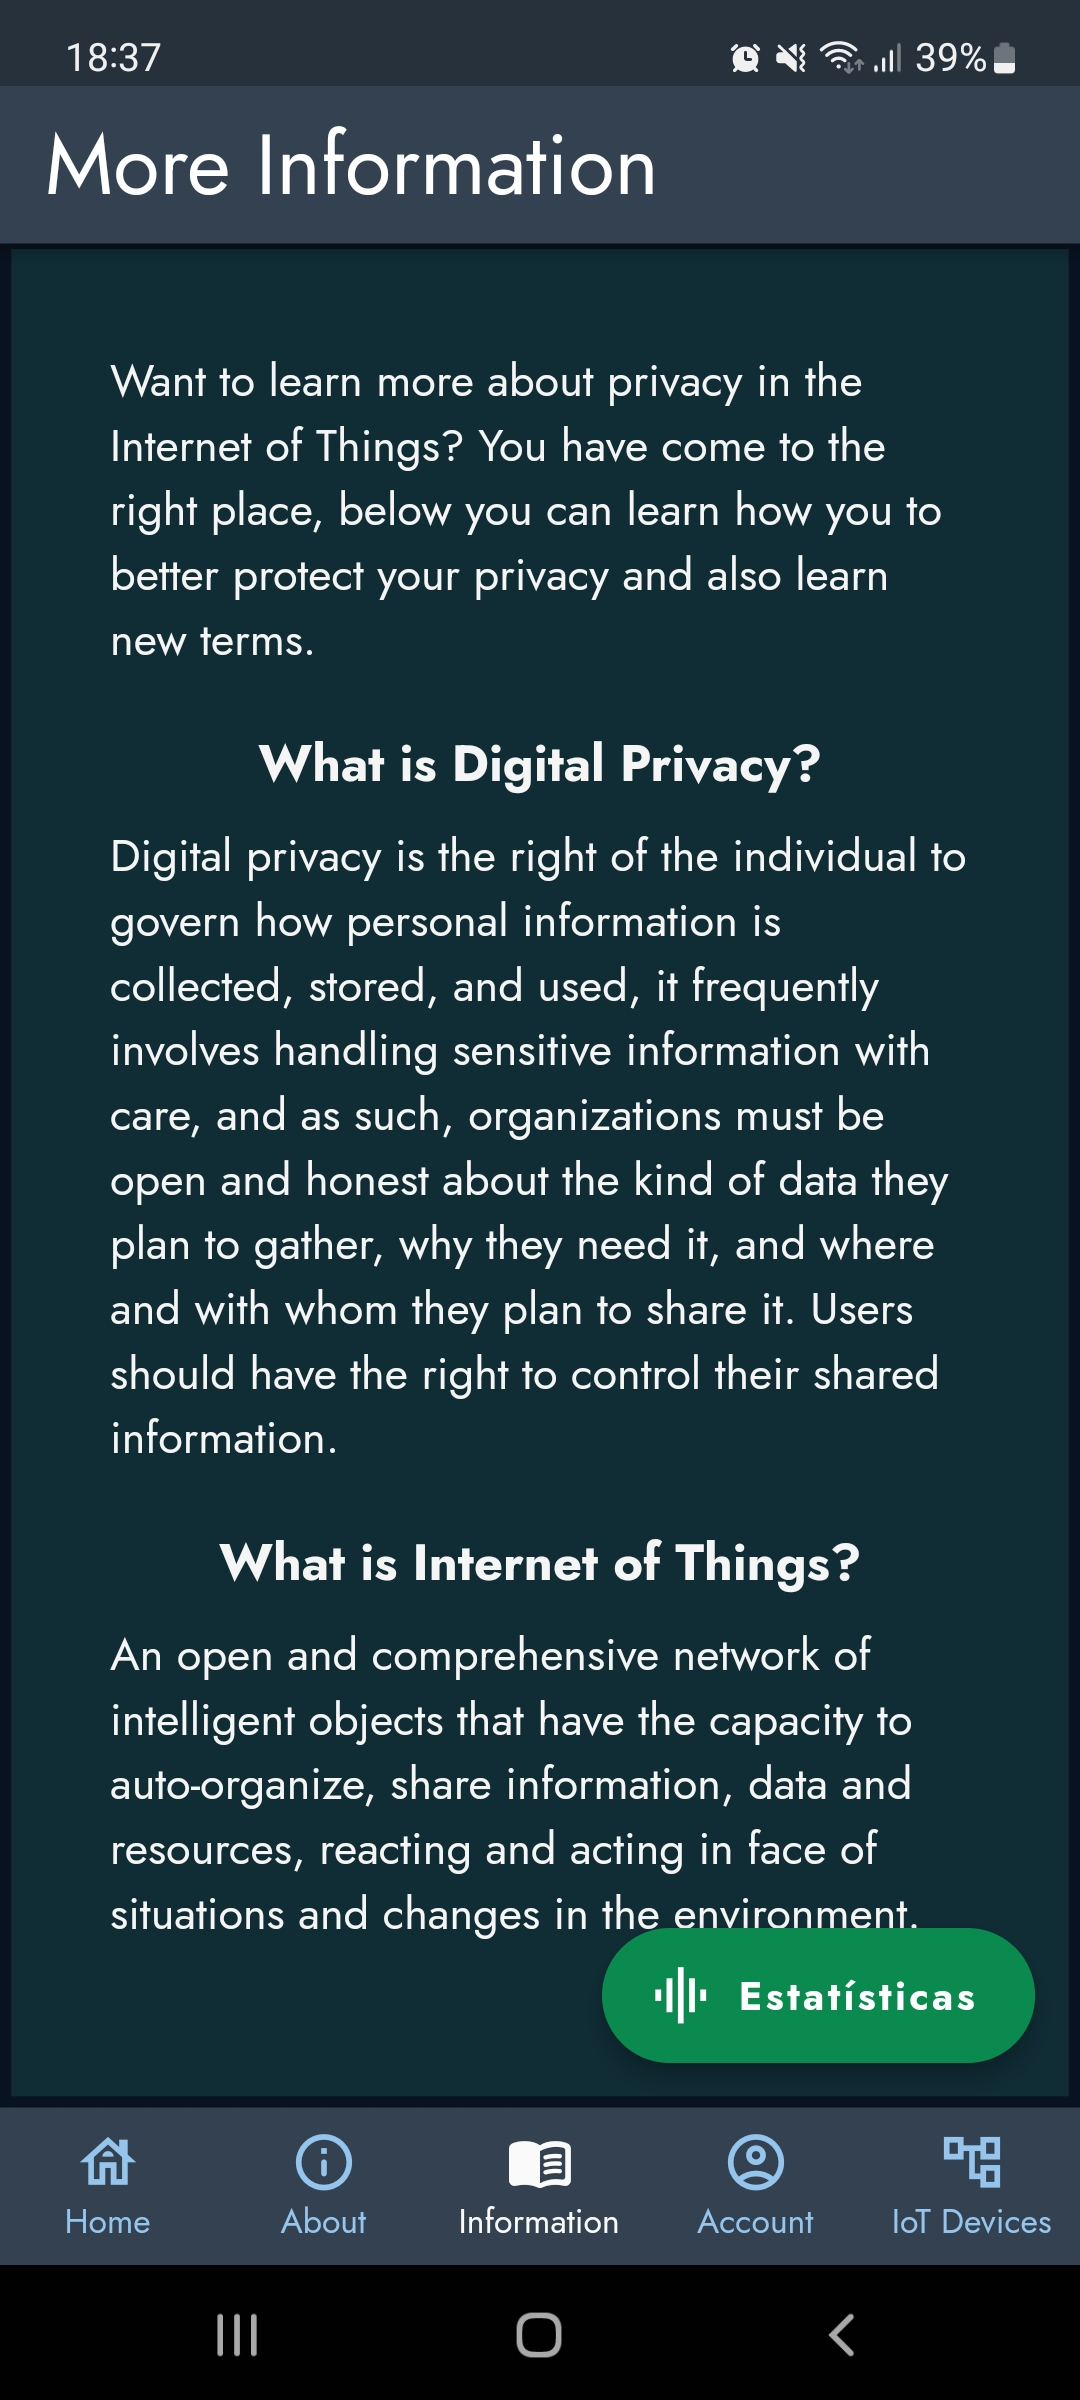
\includegraphics[width=125pt]{../assets/images/live_more_info.jpg}
        \caption{}
        \label{fig:highfaq}
    \end{subfigure}
    \begin{subfigure}{0.30\textwidth}
        \centering
        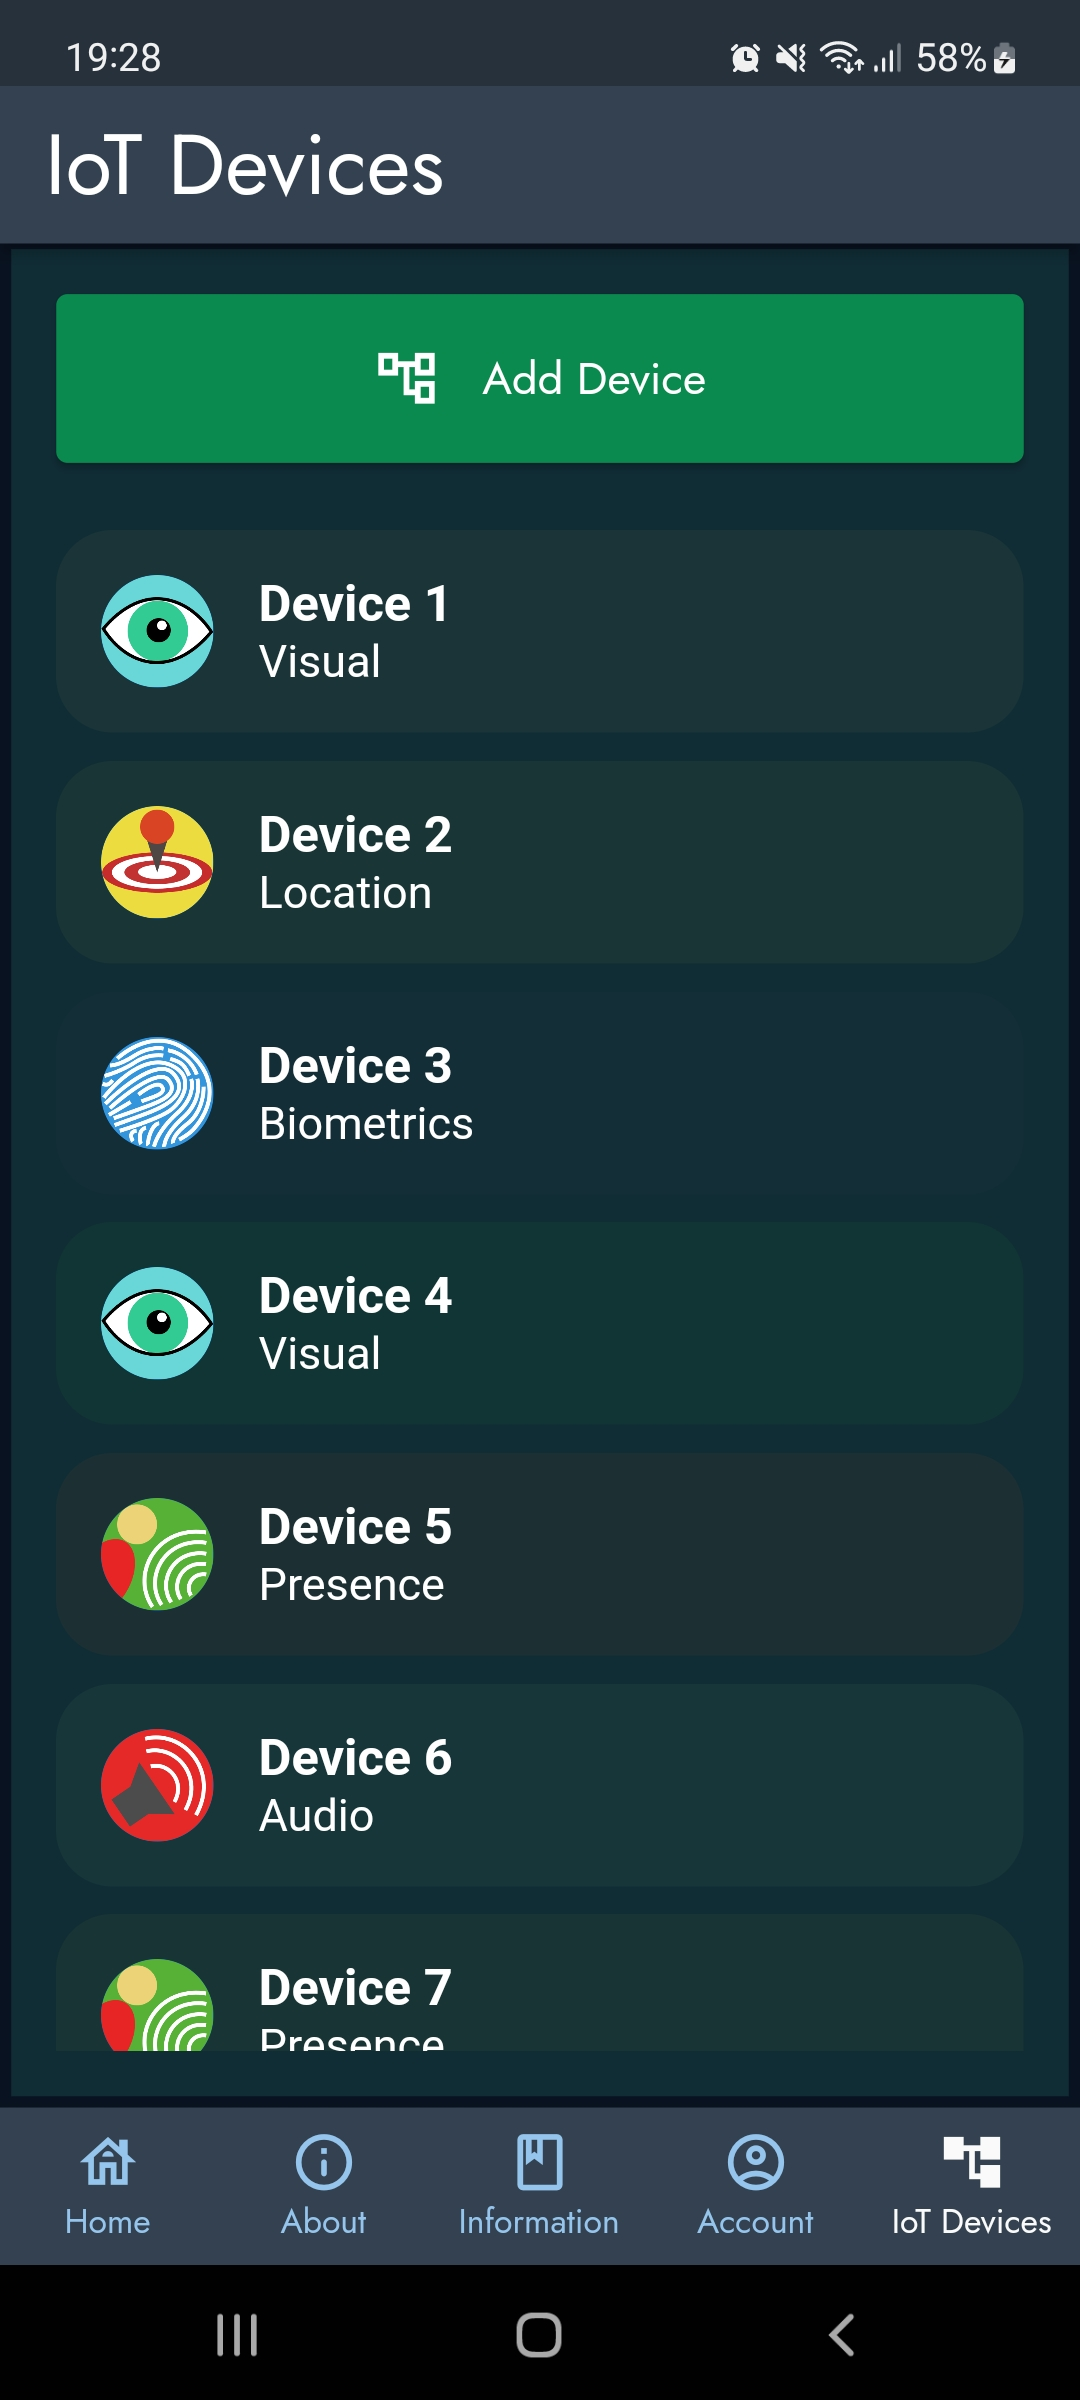
\includegraphics[width=125pt]{../assets/images/live_devices.jpg}
        \caption{}
        \label{fig:highfaq}
    \end{subfigure}
    \begin{subfigure}{0.30\textwidth}
        \centering
        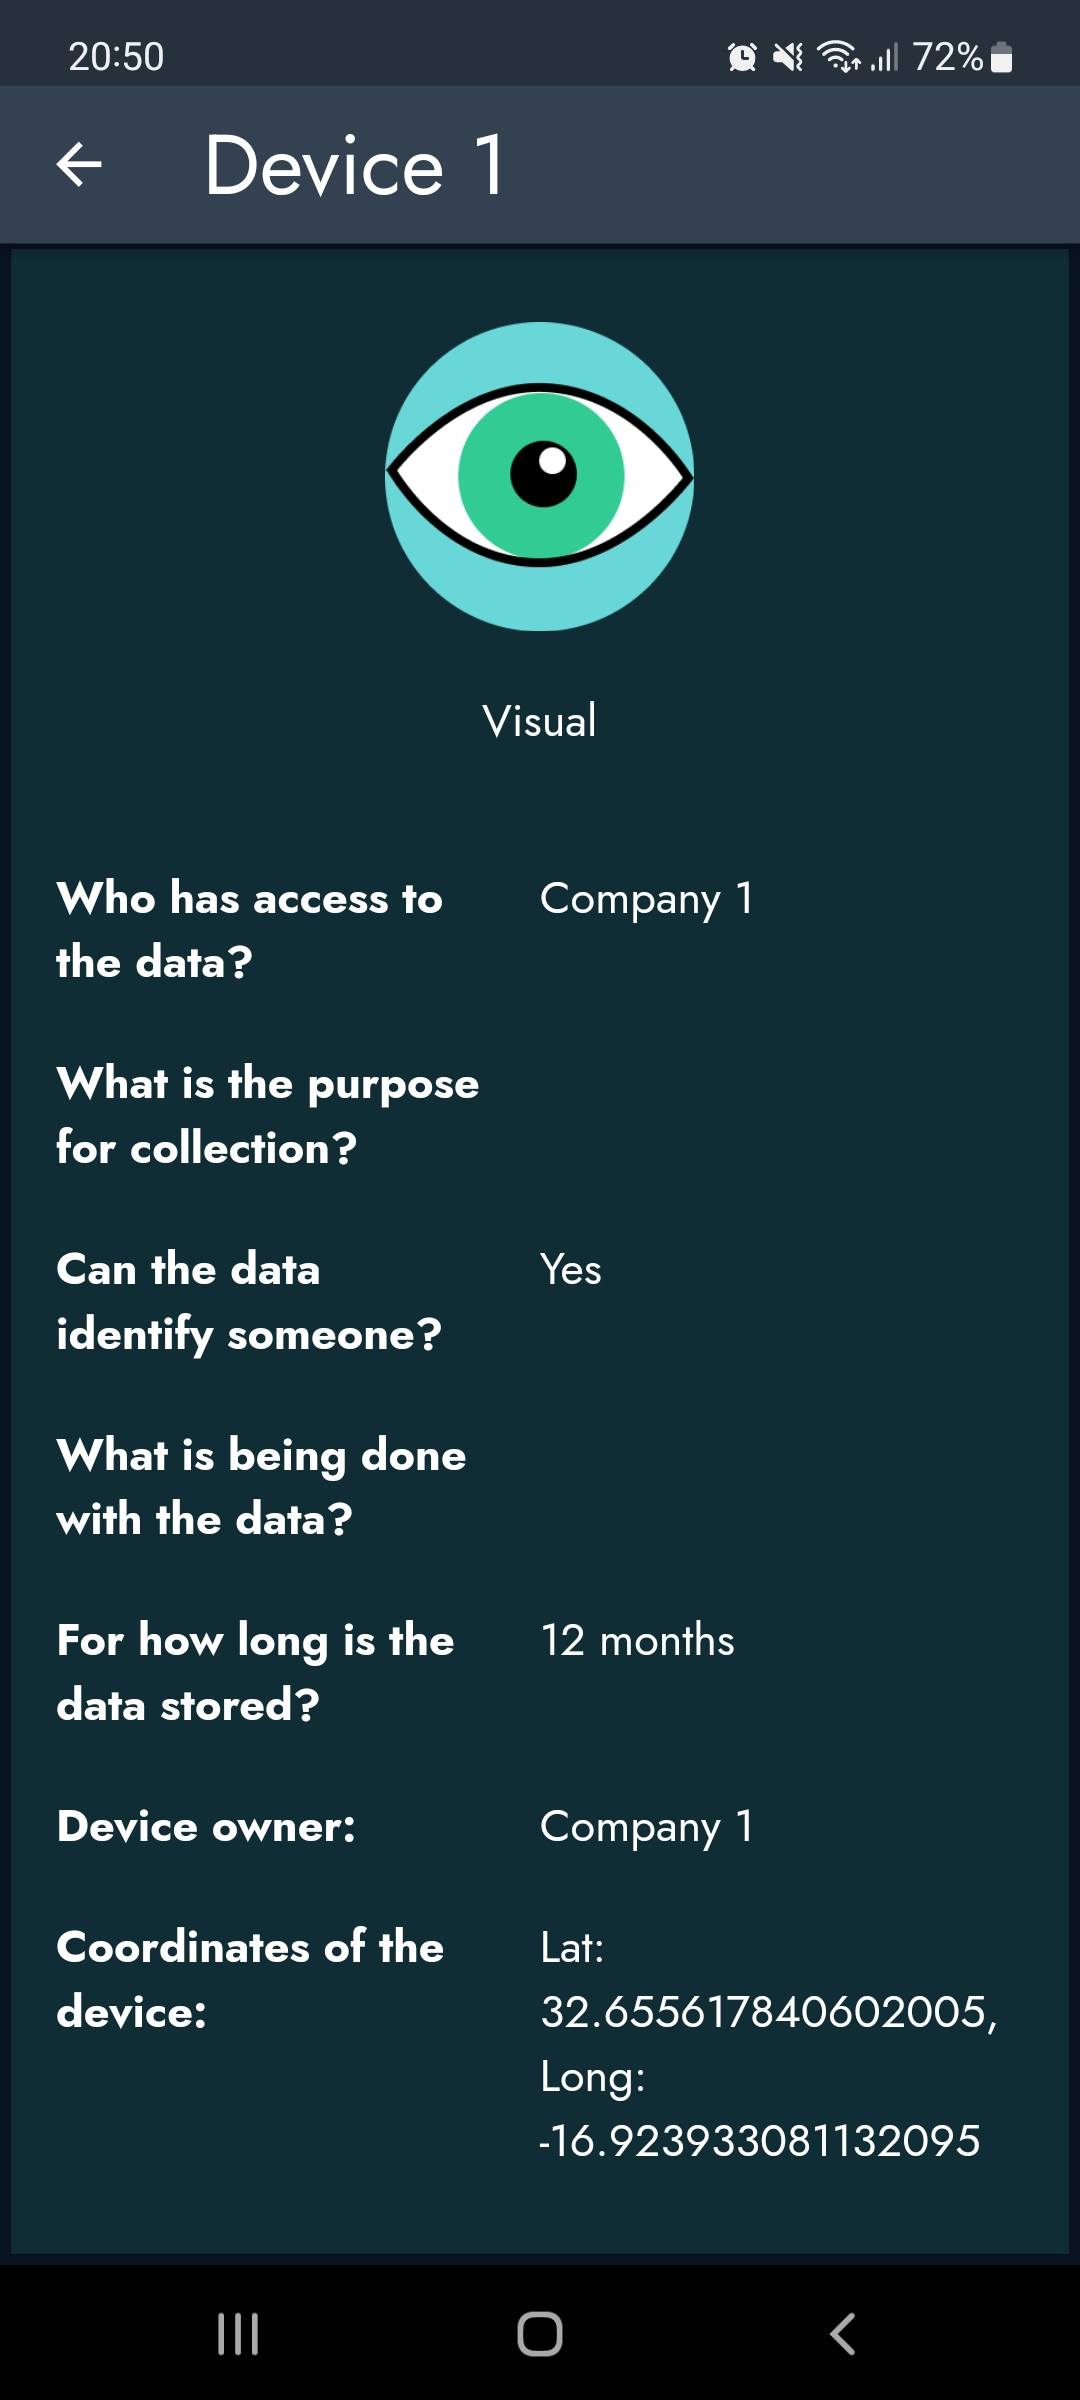
\includegraphics[width=125pt]{../assets/images/live_device_info.jpg}
        \caption{}
        \label{fig:highfaq}
    \end{subfigure}
    \begin{subfigure}{0.30\textwidth}
        \centering
        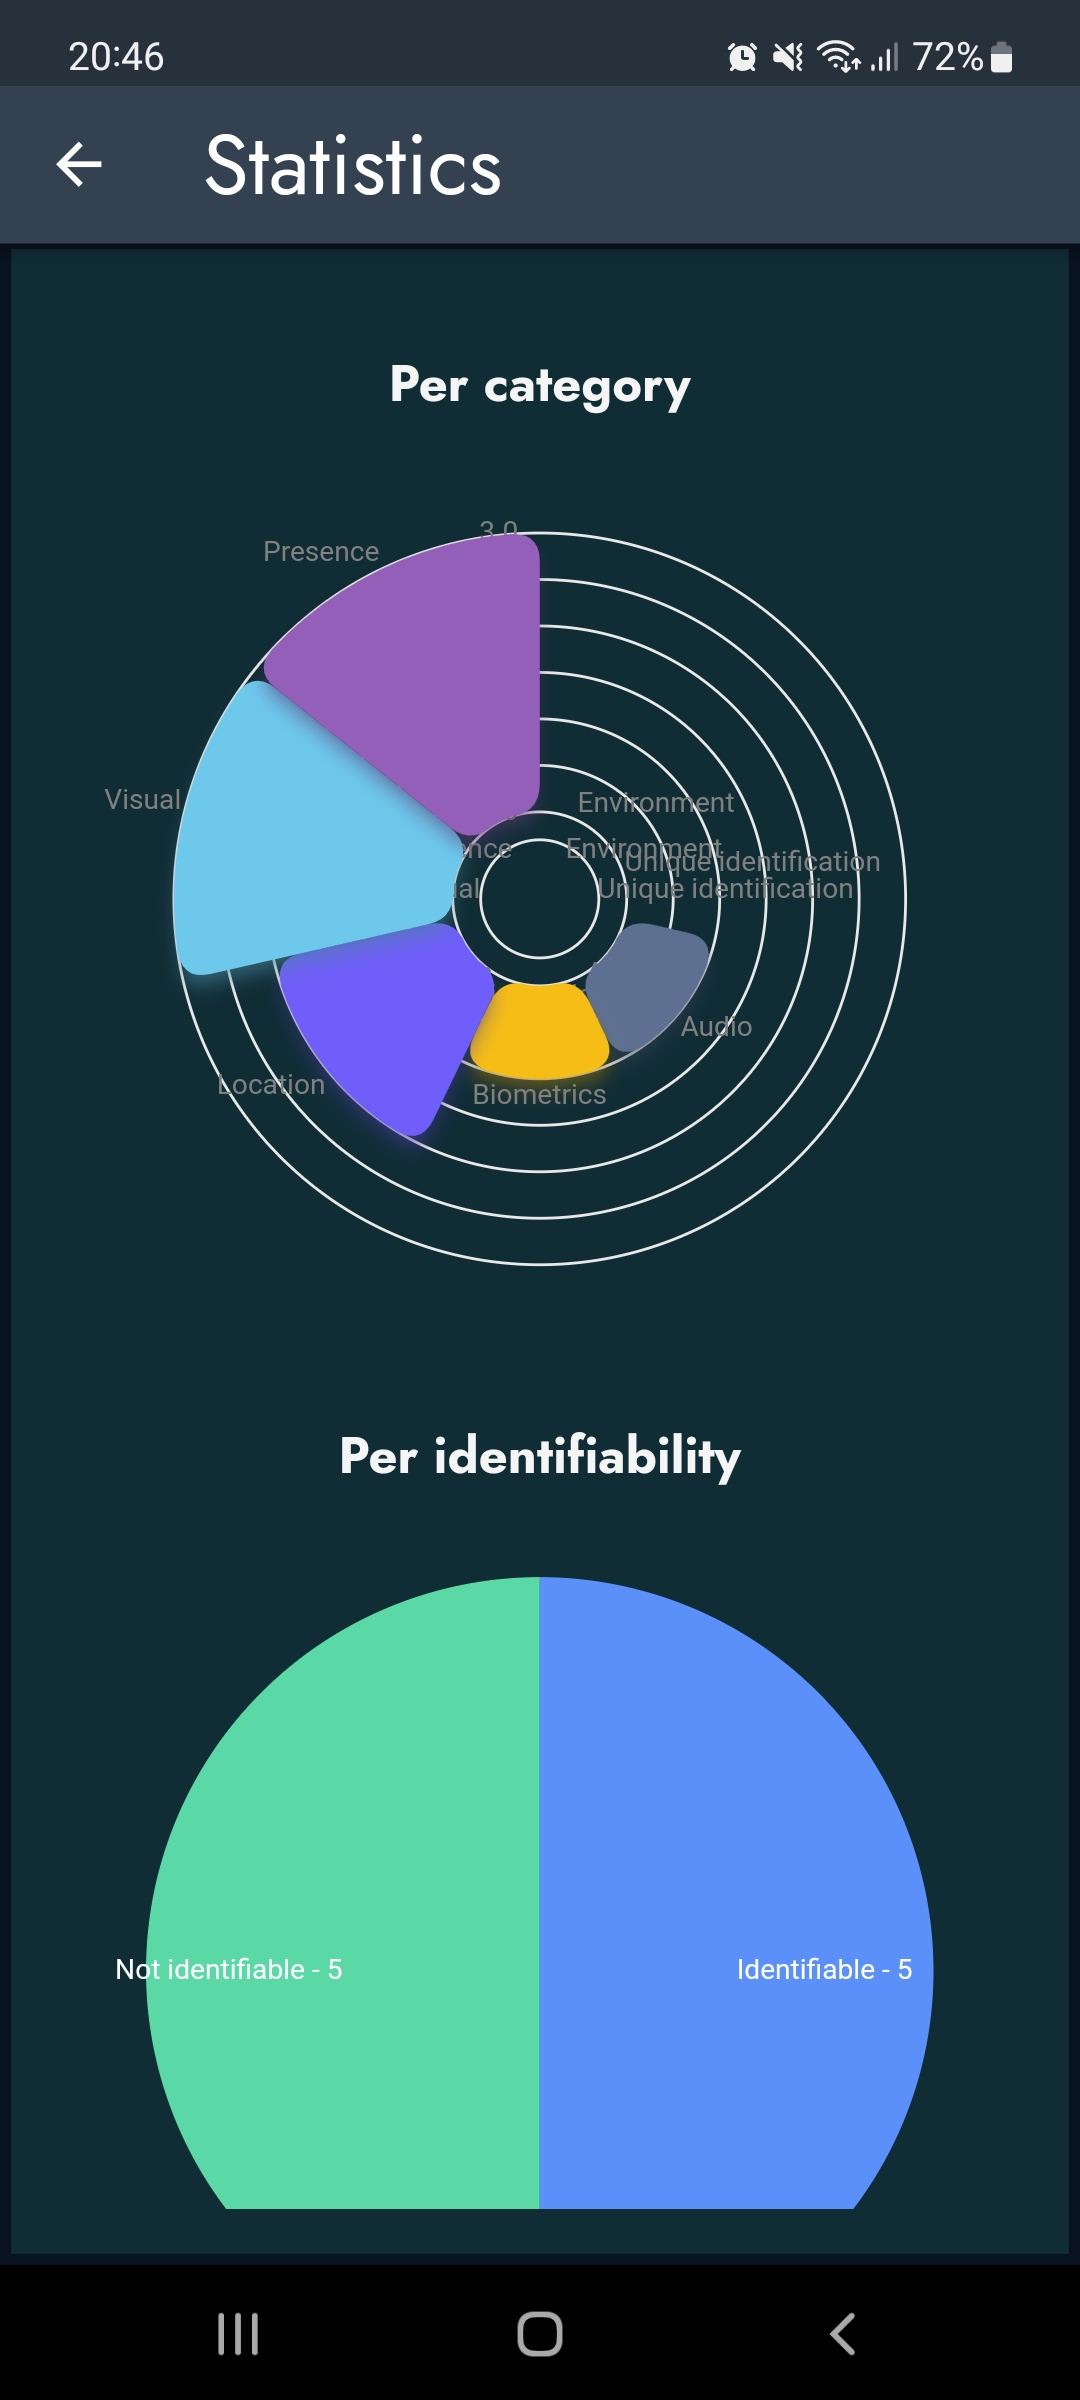
\includegraphics[width=125pt]{../assets/images/live_statistics.jpg}
        \caption{}
        \label{fig:highfaq}
    \end{subfigure}
    \caption{Live version of the application with pages: (a) homepage, (b) about, (c) FAQ, (d) devices, (e) device information and (f) statistics pages.}
    \label{fig:live_app}
\end{figure}

Usability tests were conducted in person with 7 participants of different
ages, professional fields and qualifications. Before doing the tests,
some questions were made to gather the general level of digital literacy
related to IoT and privacy, then the participants were asked to fill in the
survey, if they had not done it yet, as this gives some insight into what the
application is about. The usability tests consists of single ease questions \cite{tedesco2006comparison}
and system usability scale \cite{brooke1996sus}, as can be seen on appendix \ref{appendix:usability_tests}.
The single ease question was used after the participant performed each task, the
participant would answer how difficult they though the task was in a
scale of 1 to 7. The system usability scale was used after the participants
performed all tasks.
